\documentclass[12pt,a4paper]{report}

% --- Paquetes de Idioma y Codificación ---
\usepackage[utf8]{inputenc}
\usepackage[T1]{fontenc}
\usepackage[spanish, es-tabla]{babel}

% --- Diseño de Página ---
\usepackage{geometry}
\geometry{top=2.5cm, bottom=2.5cm, left=3cm, right=3cm}

% --- Matemáticas y Símbolos ---
\usepackage{amsmath, amssymb, amsthm}

% --- Colores y Cajas ---
\usepackage[dvipsnames]{xcolor}
\usepackage[most]{tcolorbox}

% Caption

\usepackage{caption}

% Gráficos

\usepackage{graphicx}

% Espaciadora

\newcommand{\esp}{\vspace{0.5cm}}

% promedio

\newcommand{\prom}[1]{\left\langle #1 \right\rangle}

% ket

\newcommand{\ket}[1]{| #1 \rangle}

% bra

\newcommand{\bra}[1]{\langle #1 |}

% braket

\newcommand{\braket}[2]{\langle #1 | #2 \rangle}

% Bibliografía

\usepackage[style=apa, backend=biber]{biblatex} % Estilo APA
\addbibresource{biblio.bib} % Nombre de tu archivo .bib

% Configuración de cajas personalizadas
\newtcolorbox{importante}{
	colback=red!5!white,
	colframe=red!75!black,
	title=Importante,
	fonttitle=\bfseries
}

\newtcolorbox{nota}{
	colback=blue!5!white,
	colframe=blue!75!black,
	title=Nota,
	fonttitle=\bfseries
}

% Definición de la caja de bibliografía
\newtcolorbox{bibliografia}{
	colback=gray!5!white,
	colframe=gray!75!black,
	title=Bibliografías útiles,
	fonttitle=\bfseries,
	breakable
}

% Socrative para óptica 2

\newtcolorbox{Socrative}{
	colback=orange!5!white,
	colframe=orange!75!black,
	title=Socrative,
	fonttitle=\bfseries,
	breakable
}

% Float

\usepackage{float}

% --- Hipervínculos ---
\usepackage{hyperref}
\hypersetup{
	colorlinks=true,
	linkcolor=blue,
	filecolor=magenta,      
	urlcolor=cyan,
}

% --- Datos del Documento ---
\title{Óptica II}
\author{Chengyu Jin}
\date{\today}

\begin{document}
	
	\maketitle
	
	\tableofcontents
	\newpage
	
	\chapter{Láser y LED. Principales aplicaciones}
	
	Dedicaremos este tema a dos tipos de fuentes de luz que han sido fundamentales en el desarrollo de la Óptica: el LED y el láser. La emisión del diodo emisor de luz (\textit{Light Emitting Diode}) o LED se basa en la interacción fotón electrón en semiconductores dopados, que forman uniones p-n. El primer LED fue desarrollado en torno a la misma fecha que el láser de Maiman, en 1961, por Biard y Pittman. Emitía en infrarrojo, así que no tuvo mucha aplicación práctica hasta que, en el año siguiente, Nick Holonyak desarrolló el primer LED visible (rojo). A partir de entonces, en los siguientes 20-30 años se estuvo experimentando mucho sobre materiales semiconductores para conseguir una mayor emisión y variedad de longitudes de onda, y en 1994 se produce el primer \textit{Super bright LED}, inventado por Shuji Nakamura. Desde entonces, la tecnología LED ha avanzado tanto que ha sido capaz de convertirse en la fuente de iluminación dominante en espacios interiores, y avanza fuerte también en el campo de la iluminación nocturna en espacios urbanos.
	
	\esp
	
	Láser es un acrónimo de \textit{Light Amplification by stimulated emission of radiation}. Ha supuesto una verdadera revolución en la ciencia y la tecnología de los últimos 60 años. En este tema, vamos a ver brevemente algunas bases de su funcionamiento y sus características más destacadas. Pero antes, hagamos un poco de historia. La emisión láser se basa en una forma especial de interacción luz-materia que puso de manifiesto Einstein en 1916, la emisión estimulada. Pero no fue hasta 1950 que surgió la primera realización práctica de un dispositivo basado en la emisión estimulada: fue el máser, que funciona en el rango de las microondas. Fue desarrollado gracias al trabajo de C.H. Townes, A.M. Prokhorov y N.G. Basov, entre otros. En seguida, se empieza a pensar en construir un dispositivo que funcione en el rango visible. En 1958, C.H. Townes y A.L. Shawlow realizaron un estudio teórico sobre las condiciones necesarias para ello. Y en Julio de 1960, T.H. Maiman consigue el primer prototipo de láser utilizando rubí (óxido de Cromo) como medio de interacción. Las aplicaciones de ambos tipos de fuentes son muy variadas e interesantes, como veremos en los ejemplos de las secciones del tema dedicadas a los campos de aplicación. La palabra \textit{boom} seguramente se queda corta para describir la multitud de usos que tienen los láseres y fuentes de LED en la actualidad.
	
	\section{LED}
	
	En esta sección, vamos a estudiar someramente algunas de las características más relevantes de las fuentes LED, que son en definitiva un tipo de dispositivos optoelectrónicos (fuentes y detectores basados en la interacción fotón-electrón fundamentalmente en semiconductores). Nos centraremos en las fuentes en este tema, y dentro de los basados en semiconductores, veremos los LED y también los láseres de diodo en la siguiente sección. Vamos a tratar primero algunos aspectos básicos de semiconductores, para después centrarnos en el mecanismo de funcionamiento del LED y sus características de emisión, viendo algunas de las configuraciones y dispositivos más comunes y de mayor interés.
	
	\subsection{Teoría básica de semiconductores}
	
	\begin{figure}[H]
		\centering
		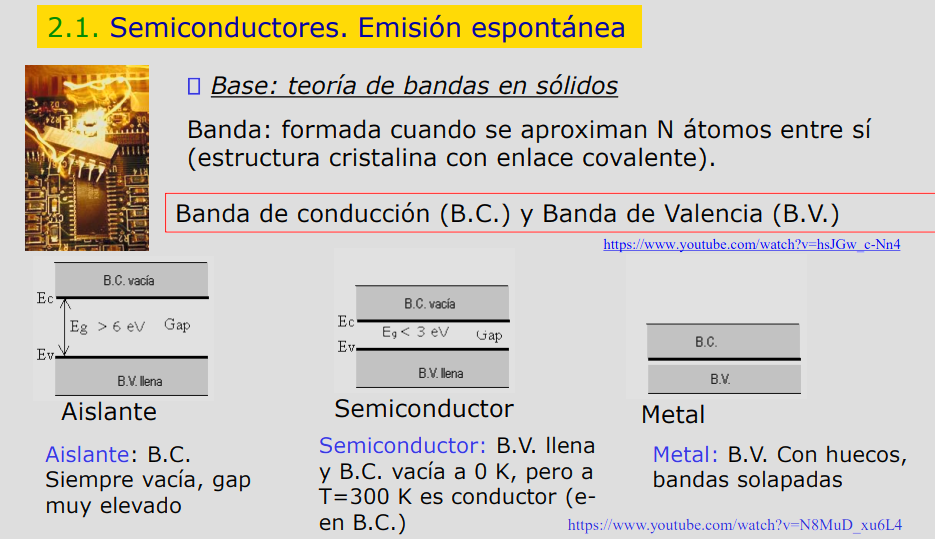
\includegraphics[width=0.7\textwidth]{IMG/led.png}
	\end{figure}
	
	\esp
	
	La base para comprender cómo funcionan los semiconductores es la teoría de bandas en sólidos. Aquí vamos a exponer de forma muy breve sólo algunos de sus aspectos más relevantes, porque es un campo muy amplio, como podrán comprobar los que tengan pensado dedicarse a la microelectrónica.
	
	\esp
	
	Los niveles de energía que pueden ocupar los electrones en átomos aislados son discretos y por lo general bastante separados (en especial los niveles inferiores de energía). Pero cuando $N$ átomos se aproximan entre sí para formar un sólido con una estructura cristalina de enlace covalente, se observa que si bien los niveles de energía de los electrones más internos no se ven afectados apreciablemente por la presencia de átomos vecinos, en cambio, los niveles energéticos más externos sufren modificaciones importantes, ya que estos electrones están siendo compartidos por varios átomos en la estructura cristalina. El acoplamiento entre las capas más externas de electrones de estos átomos da como resultado una banda de estados de energía muy próximos entre sí, en lugar de los niveles más separados propios del átomo aislado. Los niveles formados como consecuencia de este acoplamiento constituyen una banda casi continua de energía entre sus extremos inferior y superior. A la banda correspondiente a niveles de menor energía se denomina \textit{banda de valencia} (B.V.), y a la banda de niveles superiores se llama \textit{banda de conducción} (B.C.). Entre ambas bandas, queda un hueco de energía que no puede ser ocupado por los electrones, y se denomina \textit{gap} o salto.
	
	\esp
	
	La configuración de las bandas condiciona el comportamiento del material. Por ejemplo, en un aislante, la B.V. está llena y la B.C. vacía, porque el gap (mayor de 6 eV) es muy elevado y no pueden acceder los electrones a la B.C. En un metal, las bandas de conducción y valencia están solapadas, con lo que es posible siempre la movilidad de los electrones hacia la B.C. El que los electrones puedan acceder a la B.C. condiciona el que el material pueda conducir la corriente eléctrica o no. En los semiconductores, el gap es pequeño entre ambas bandas, pero no están confundidas como en los metales, con lo cual a $T = 0$K tienen la B.C. vacía, comportándose como aislantes. Pero a temperatura ambiente (300K), por agitación térmica u otros procesos, los electrones adquieren energía suficiente para saltar el gap y pasar a la B.C., con lo cual se comportan como conductores.
	
	\esp
	
	\begin{figure}[H]
		\centering
		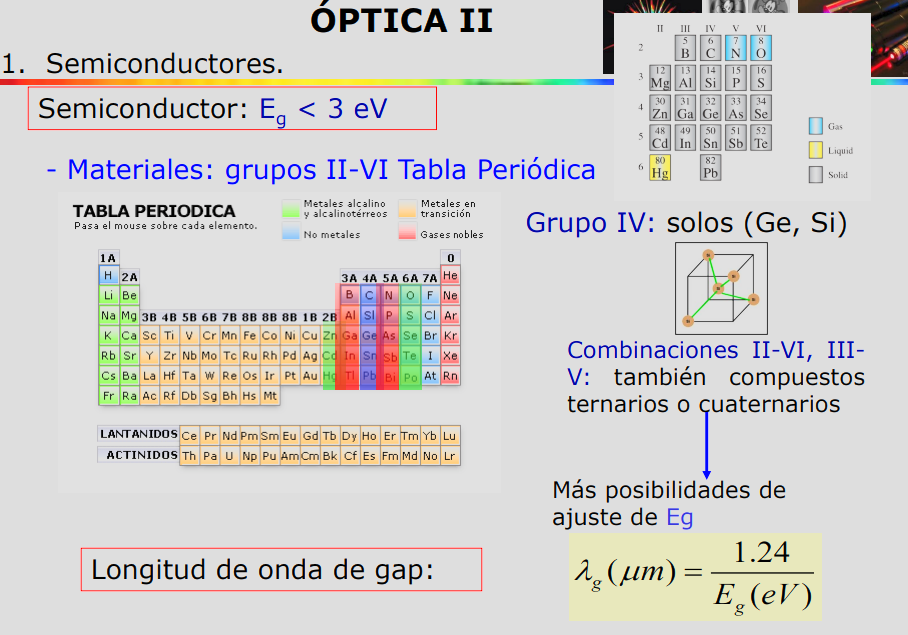
\includegraphics[width=0.7\textwidth]{IMG/led2.png}
	\end{figure}
	
	\esp
	
	Se considera que un material es semiconductor si el valor del gap no excede los $3eV$ (ver el esquema en la figura 1).
	
	\esp
	
	\begin{figure}[H]
		\centering
		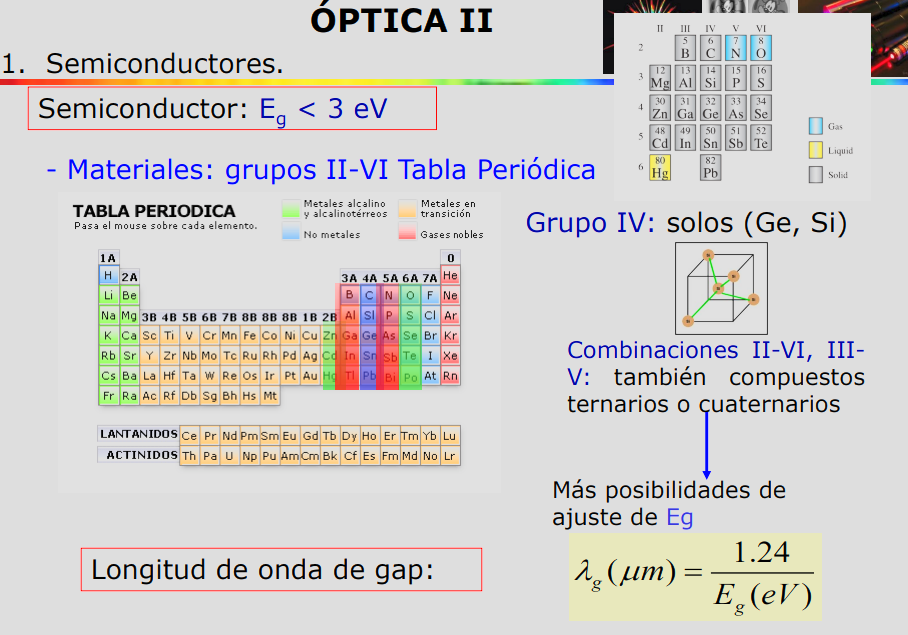
\includegraphics[width=0.7\textwidth]{IMG/led2.png}
	\end{figure}
	
	\esp
	
	Los materiales semiconductores están formados por elementos de los grupos $II$-$VI$ de la Tabla periódica. Los del grupo $IV$, como el germanio ($Ge$) o silicio ($Si$), pueden funcionar como semiconductores por sí mismos; los de los grupos $III$ y $V$, necesitan formar compuestos, igual que los de los grupos $II$ y $VI$. Los compuestos pueden ser binarios (por ejemplo, $GaAs$ o Arseniuro de Galio), ternarios ($InGaAs$) o incluso cuaternarios, lo que ofrece mayores posibilidades de ajuste para el valor de la energía de gap.
	
	\esp
	
	Los semiconductores se caracterizan, entre otros parámetros, por la longitud de onda de gap correspondiente (longitud de onda en el vacío correspondiente a la frecuencia de la transición de mínima energía entre las bandas de conducción y valencia). Se obtendría entonces considerando que la energía del gap es: $E_g = h\nu$, y a su vez, $\lambda = \frac{c}{\nu} = \frac{ch}{E_g} = \frac{1.24}{E_g}$, si expresamos $E_g$ en $eV$, y la longitud de onda quedaría entonces en micras.
	
	\esp
	
	Vamos a ver ahora brevemente cómo se produce la interacción fotón-electrón en este tipo de materiales. Hay dos procesos fundamentales: absorción de fotones para producir saltos de electrón a la B.C., con lo que se crean huecos en la B.V. (lo que se llama \textit{creación de pares electrón-hueco}), y el proceso contrario de emisión de fotones cuando un electrón pasa a ocupar un hueco de la B.V. (\textit{recombinación radiativa}). Hay que tener en cuenta que no todas las recombinaciones son radiativas. La emisión puede ser espontánea o estimulada si se dan las condiciones para ello, lo que puede dar lugar a fuentes láser basadas en semiconductores.
	
	\esp
	
	\begin{figure}[H]
		\centering
		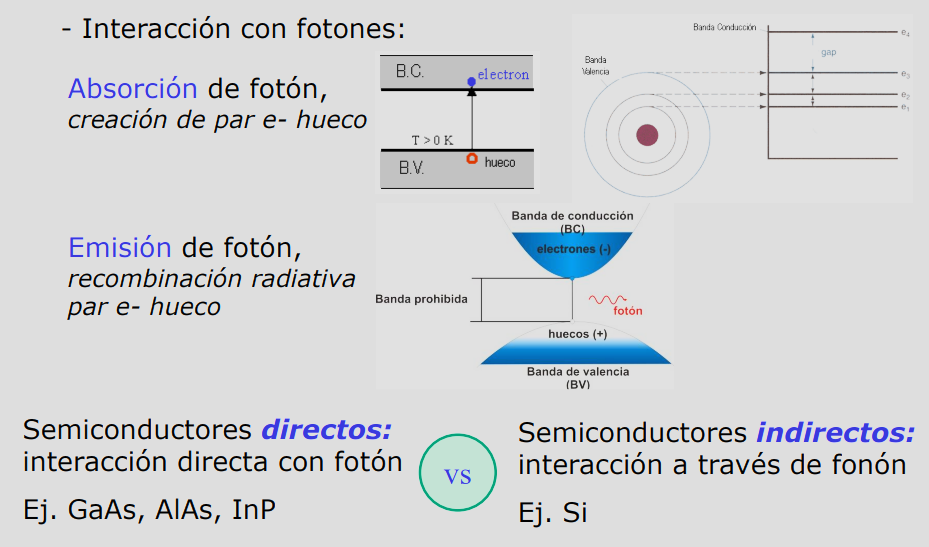
\includegraphics[width=0.7\textwidth]{IMG/led4.png}
	\end{figure}	
	
	\esp
	
	Desde el punto de vista de la interacción con los fotones, distinguimos dos tipos de semiconductores: los \textbf{directos}, en los que se dan los procesos que hemos descrito, como el $AlAs, GaAs, InP, ZnS$ y otros. Son por tanto los adecuados para constituir la base de fuentes de luz. También hay otro tipo de semiconductores en los cuales la interacción directa es con fonones (que son las partículas asociadas con el transporte de energía en ondas mecánicas y sonoras según la teoría cuántica), de forma que para que se produzca una emisión de un fotón deben convivir simultáneamente las tres partículas (electrón, fonón y fotón), con lo cual la probabilidad de recombinación radiativa es bastante menor. 
	
	\esp
	
	\begin{figure}[H]
		\centering
		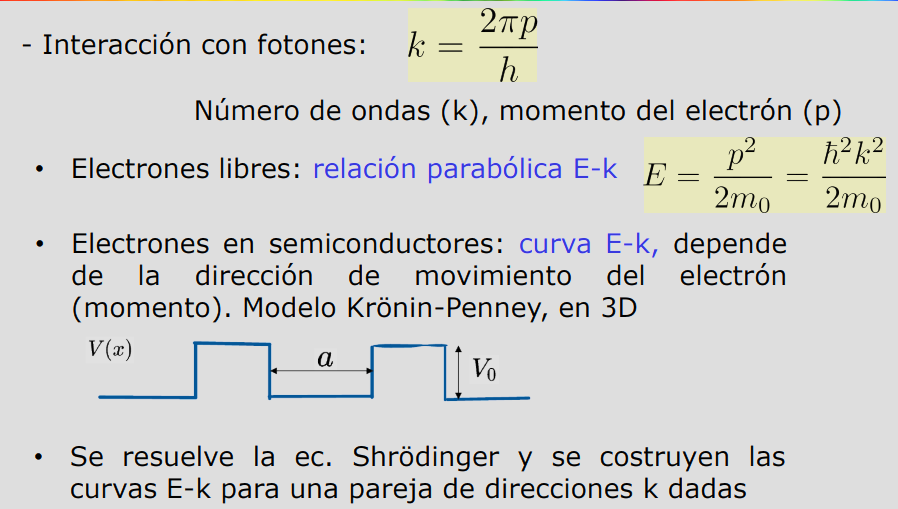
\includegraphics[width=0.7\textwidth]{IMG/led5.png}
	\end{figure}
	
	\esp
	
	Son los llamados \textbf{semiconductores indirectos}, como el $Si$. Para saber si un material es de tipo directo o indirecto, hace falta conocer su curva $E-k$ (relación energía-número de onda). El número de onda se relaciona con el momento del electrón, según $k = \frac{2\pi p}{h}$. Entonces, por ejemplo, para un electrón no ligado, la energía del electrón y el número de onda presentan una relación de tipo parabólico, ya que se cumple que:
	
	\esp
	
	\begin{equation}
		E = p^2 / 2m_0 = \hbar^2 k^2 / 2m_0
	\end{equation}
	
	\esp
	
	\begin{figure}[H]
		\centering
		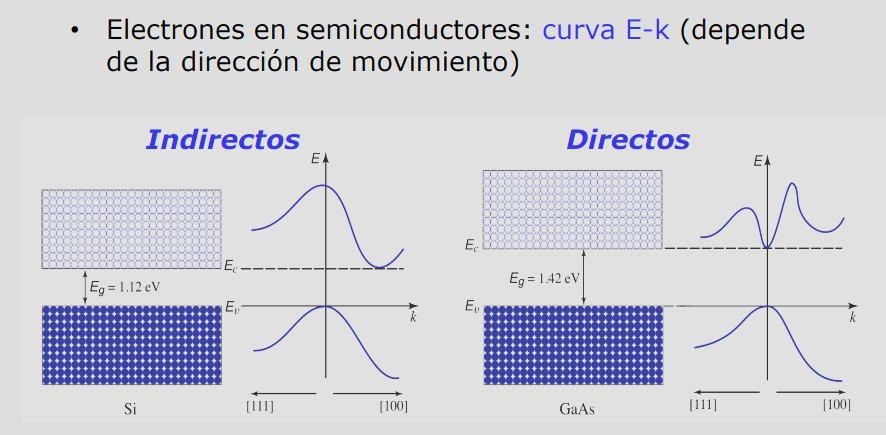
\includegraphics[width=0.7\textwidth]{IMG/led6.png}
	\end{figure}
	
	\esp
	
	En el caso de electrones (o huecos) en semiconductores, resolviendo la ecuación de Schrödinger asociada a una simplificación de la función potencial como una función periódica... se llega a que la energía es una función periódica de las tres componentes del vector $k$, que serían $(k_1, k_2, k_3)$, y las constantes de periodicidad dependen de tres variables típicas que caracterizan la estructura cristalina del compuesto. Entonces, la energía de un electrón no depende sólo del módulo de su momento, sino también de su dirección de movimiento. Esto se puede ilustrar con el diagrama $E-k$, como se muestra en la figura 2 para los casos de $GaAs$ y $Si$.
	
	\esp
	
	\begin{figure}[H]
		\centering
		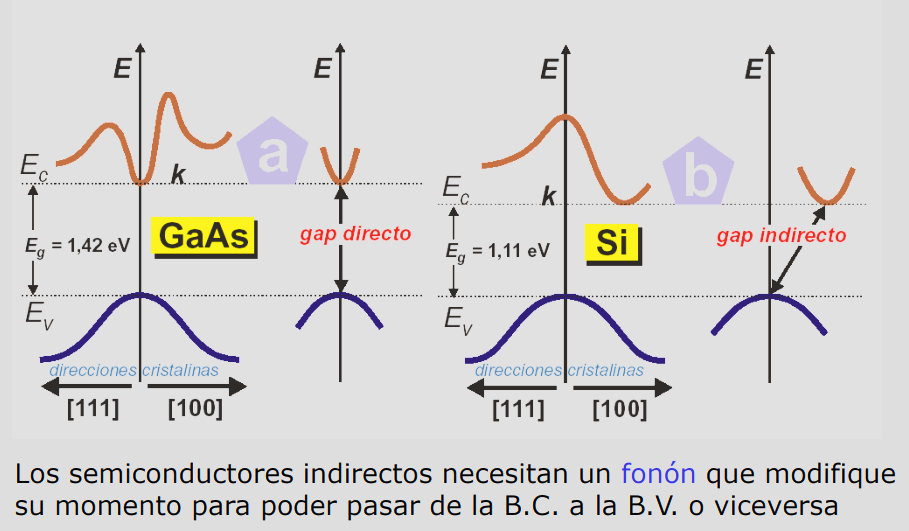
\includegraphics[width=0.7\textwidth]{IMG/led7.png}
	\end{figure}
	
	\esp
	
	Justo en la zona más alta de la banda de valencia, y en la zona más baja de la banda de conducción, las curvas $E - k$ pueden aproximarse por parábolas, y esto nos daría una \textit{masa efectiva} para los huecos y electrones respectivamente. Pero lo que más nos interesa de estas curvas es que vemos que, en el caso de los semiconductores \textit{directos}, como el $GaAs$, el valor mínimo de gap entre las bandas se da para un mismo valor de número de onda (máximo y mínimo de las curvas $E - k$ alineados), mientras que para los materiales \textit{indirectos}, como el $Si$, es necesario para el electrón cambiar su valor de momento para poder realizar la transición, porque los niveles máximo y mínimo de las dos bandas no están alineados. Por eso, los materiales indirectos necesitan de la interacción con otra partícula adicional (el \textit{fonón}) para cambiar el momento del electrón y permitir su transición a la banda de conducción, mientras que no es necesaria la intervención de los fonones en el caso de los materiales directos.
	
	\subsection{Dopaje. Uniones p-n.}
	
	\begin{figure}[H]
		\centering
		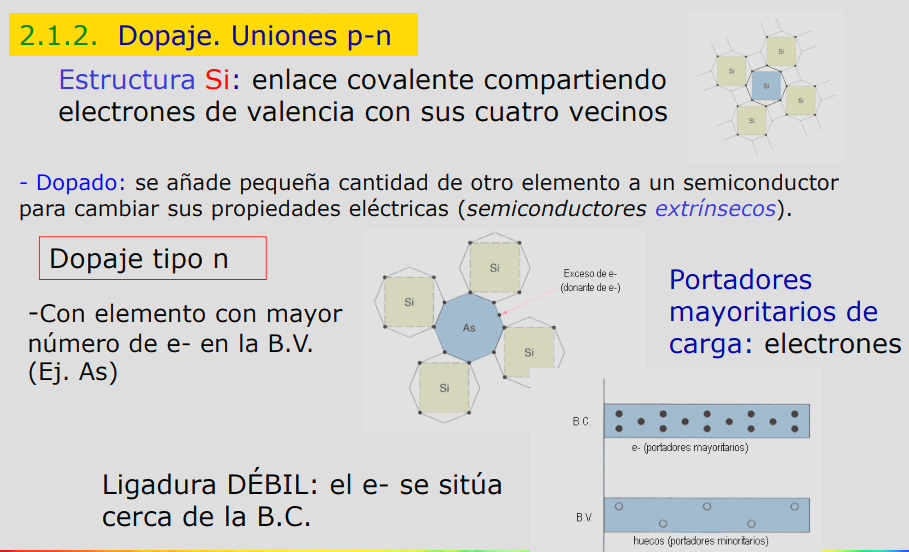
\includegraphics[width=0.7\textwidth]{IMG/led8.png}
	\end{figure}
	
	\esp
	
	En muchas ocasiones, se añade a los semiconductores una pequeña cantidad de otro elemento semiconductor, lo que permite cambiar profundamente sus propiedades ópticas y eléctricas. Este proceso se llama dopado o dopaje. Hay dos categorías principales de compuestos dopados: los \textit{tipo p} y los \textit{tipo n}. Para entender su estructura, vamos a tomar como ejemplo el $Si$, del grupo $IV$ y por tanto con cuatro electrones en su B.V. En estado puro, el $Si$ comparte estos electrones con otros átomos de $Si$ situados a su alrededor.
	
	\esp
	
	En los compuestos dopados \textit{tipo n}, cambiamos algunos átomos de $Si$ en la red por otros de un elemento con mayor número de electrones de valencia, como el $As$ que tiene cinco (pertenece al grupo $V$). Entonces, si cada átomo de $As$ comparte cuatro electrones con cuatro átomos de $Si$ vecinos, le queda un electrón sin compartir, débilmente ligado. Por lo tanto, el compuesto es un potencial donante de electrones. Estos electrones débilmente ligados se sitúan cerca de la B.C. del material, y constituyen los portadores mayoritarios de carga del compuesto.
	
	\esp
	
	\begin{figure}[H]
		\centering
		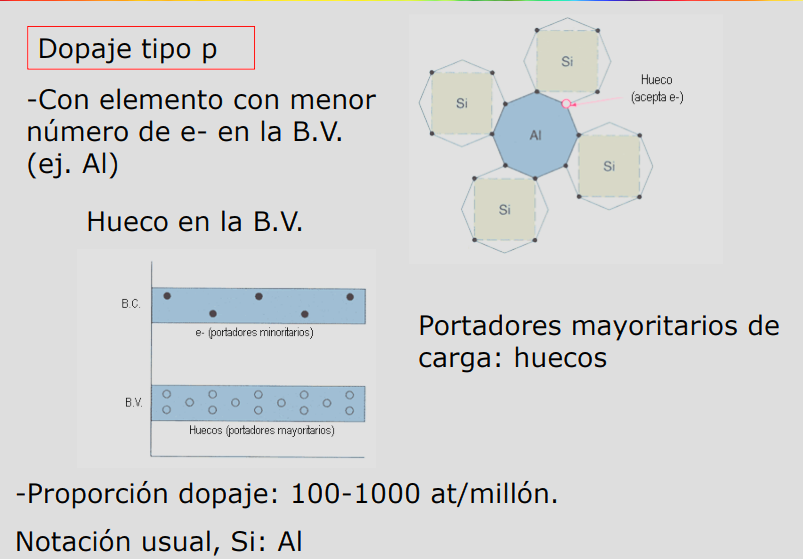
\includegraphics[width=0.7\textwidth]{IMG/led9.png}
	\end{figure}
	
	\esp
	
	En los compuestos dopados \textit{tipo p}, la estrategia es la contraria: sustituimos algunos de los átomos en este caso de $Si$ por otro elemento con menos electrones de valencia (por ejemplo, el $Al$, que tiene tres), con lo cual se crea un defecto de electrones en la red (uno de los cuatro vecinos del cada átomo de $Al$ no puede compartir electrones) y a este defecto se denomina \textit{hueco}. Los movimientos de electrones dentro del material pueden verse de forma equivalente como movimientos de huecos: cuando un electrón pasa a ocupar un hueco, el hueco cambia de posición a la anterior que ocupaba el electrón. Estos compuestos son potencialmente receptores de electrones, y tienden a cargarse negativamente. Los portadores mayoritarios de carga serían en este caso los huecos, según lo hemos explicado.
	
	\esp
	
	La proporción de dopante suele ser de 100-1000 átomos por cada millón de átomos de compuesto puro. Se notan con dos puntos tras el compuesto puro y a continuación el elemento dopante. Por ejemplo, $GaAs:Ge$ (arseniuro de galio dopado con germanio), o $Ge:B$ (germanio dopado con boro).
	
	\esp
	
	\begin{figure}[H]
		\centering
		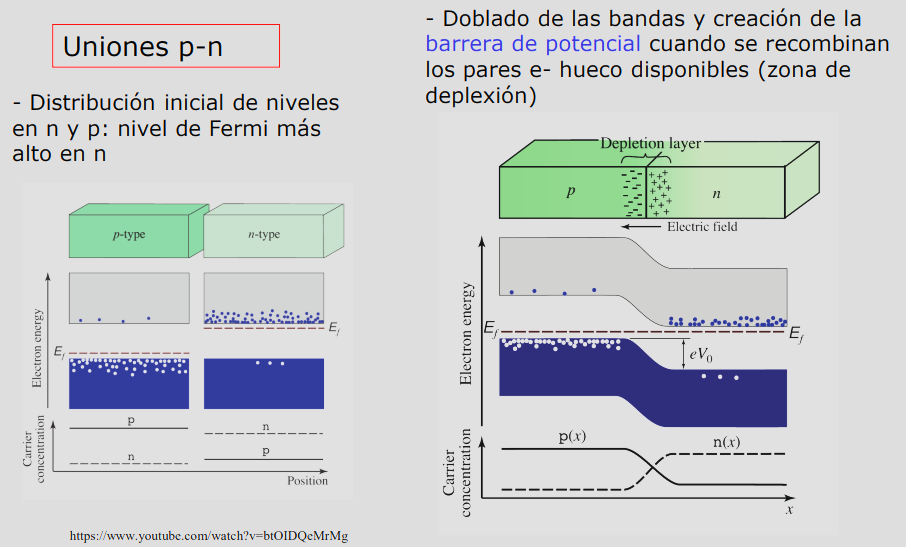
\includegraphics[width=0.7\textwidth]{IMG/pn.png}
	\end{figure}
	
	\esp
	
	Las \textit{uniones p-n} son uno de los dispositivos más útiles y eficaces en optoelectrónica. Se forman por contacto de un semiconductor dopado \textit{tipo p} con otro dopado de \textit{tipo n}, bien del mismo material puro con distinto dopante (\textit{homounión}), o de distintos materiales semiconductores (\textit{heterounión}). En la figura 3, podemos ver esquemas de materiales de ambos tipos, y cómo la distribución de niveles (bandas) del \textit{tipo n} está a un nivel de energía diferente que en el \textit{tipo p}.
	
	\esp
	
	En la figura 3, vemos representados los niveles de Fermi correspondientes a ambos materiales, que muestran cómo los electrones del \textit{tipo n} se sitúan un poco por debajo de la B.C. y los del \textit{tipo p} un poco por encima de la B.V. El nivel de Fermi se define como el nivel energético para el cual, examinando la distribución de los electrones de un material en los diferentes niveles de energía, encontraríamos un 50 por ciento de la población en niveles superiores y el restante 50 por ciento en niveles inferiores. Dado que los electrones del semiconductor dopado \textit{tipo n} están más cerca de la banda de conducción, su nivel de Fermi es superior al del material dopado \textit{tipo p}, que tiene bastantes menos electrones en dicha banda. Al poner en contacto mediante una unión metalúrgica o cristalina el material \textit{tipo p} con el \textit{tipo n}, se produce un doblado de las bandas debido a la necesidad de continuidad en el material y a la diferencia de niveles energéticos que hemos esquematizado. También se crea una barrera de potencial, proceso que vamos a ver un poco más despacio. Como resultado de este proceso, el lado \textit{tipo p} próximo a la unión queda cargado negativamente, el lado \textit{tipo n} próximo a la unión positivamente y se genera un campo eléctrico en dirección de $n$ a $p$. En la \textit{unión p-n}, se crean tres zonas claramente diferenciadas: unión, lado $p$ y lado $n$. En la zona central de la unión, los electrones y huecos quedan muy próximos, y se producen las recombinaciones posibles entre ellos, o la creación de nuevos pares. Cuando todos los pares se recombinan, se crea una zona libre de portadores de carga que se comporta como una barrera aislante: la \textit{zona de deplexión}. Los electrones abandonan el lado $n$ hacia la zona de deplexión, dejándolo cargado positivamente. Los huecos abandonan el lado $p$ hacia la zona de deplexión, dejando al lado $p$ cargado negativamente.
	
	\esp
	
	\begin{figure}[H]
		\centering
		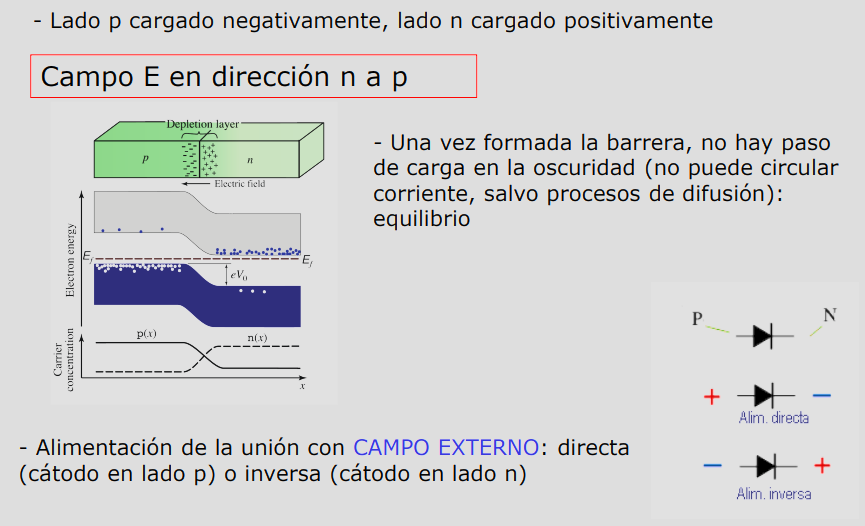
\includegraphics[width=0.7\textwidth]{IMG/pn2.png}
	\end{figure}
	
	\esp
	
	Se crea entonces el campo en dirección $n$ a $p$, que impide el paso de electrones desde $n$ y de huecos desde $p$. Aunque se recubra la unión con un conductor, no hay paso de carga porque la barrera lo impide, en ausencia de campo eléctrico externo y de interacciones con fotones, salvo procesos muy poco importantes de difusión de cargas.
	
	\esp
	
	Dado que la unión p-n es globalmente neutra (el campo interno se crea por una redistribución de carga), el campo global es también nulo en el dispositivo, lo cual se debe a que el campo interno se compensa con el creado en las zonas de contacto con los metales que van a formar parte del circuito externo que siempre llevan acoplados estos dispositivos. Una unión $p$-$n$ puede alimentarse con una diferencia de potencial adicional aplicada con dos tipos de polaridad: directa e inversa, lo que condiciona su comportamiento. En la figura vemos el símbolo estándar de las uniones $p$-$n$, y las dos polaridades de alimentación. 
	
	\esp
	
	\begin{figure}[H]
		\centering
		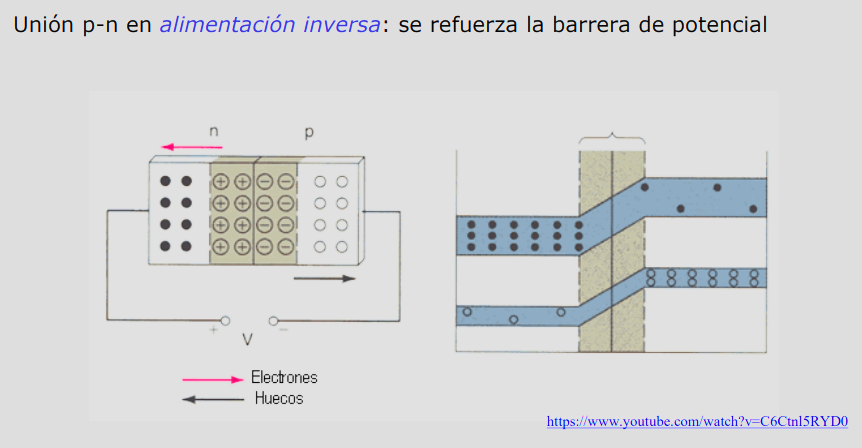
\includegraphics[width=0.7\textwidth]{IMG/pn3.png}
	\end{figure}
	
	\esp
	
	Si se aplica la polaridad inversa, es decir, se coloca el polo positivo en el lado $n$ y el polo negativo en el lado $p$, lo que hacemos es reforzar el campo existente en la unión, que actúa de barrera de potencial, por lo que no habrá paso de corriente al circuito externo en nuestras condiciones de trabajo (oscuridad). 
	
	\esp
	
	\begin{figure}[H]
		\centering
		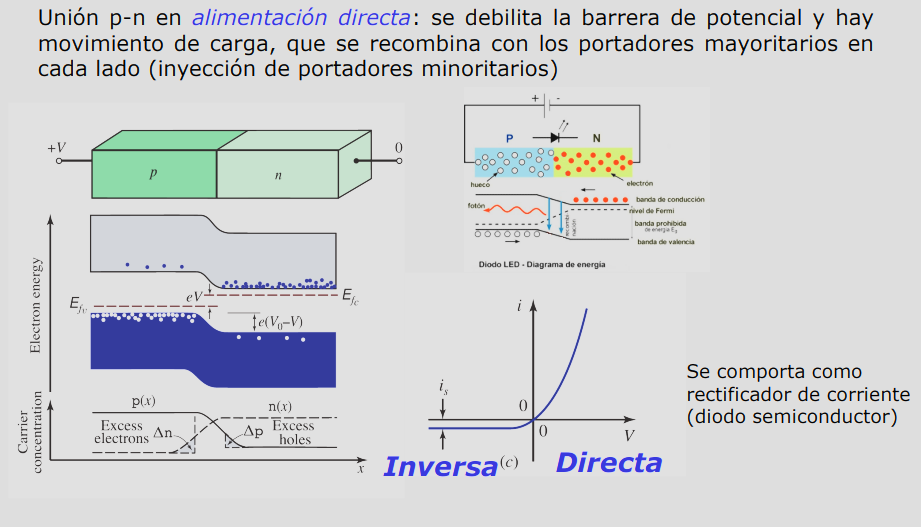
\includegraphics[width=0.7\textwidth]{IMG/pn4.png}
	\end{figure}
	
	\esp
	
	Si por el contrario se aplica la polaridad directa (polo positivo en el lado $p$ y polo negativo en el lado $n$), se crea un campo que contrarresta la barrera de potencial, y permite de nuevo el paso de electrones desde $n$ y de huecos desde $p$ a la zona de deplexión, con lo que hay cargas circulantes y el dispositivo genera corriente. El dispositivo se comporta entonces como un rectificador de corriente o diodo, y se denomina usualmente fotodiodo. 
	
	\esp
	
	Veamos ahora qué sucede si se ilumina el diodo, permitiendo que incidan fotones en la zona de deplexión y generen pares electrón-hueco. Entonces se puede producir de nuevo movimiento de cargas, como en la situación inicial del diodo antes de crearse la barrera de potencial, con lo que incluso sin alimentación externa hay una intensidad de corriente generada (movimiento de electrones desde la zona de deplexión hacia $n$, y de huecos hacia $p$). Si el diodo está iluminado, se produce un desplazamiento de la curva de intensidad frente a voltaje. A la transformación de fotones en corriente (diferencia de potencial) se denomina \textit{efecto fotovoltaico}, y se utiliza directamente en los detectores de luz. Si, por el contrario, queremos que la unión $p$-$n$ funcione como fuente de luz, debemos alimentarla con voltaje de forma directa, para contrarrestar el campo propio de la unión $p$-$n$, y obtener como resultado recombinaciones radiativas tras la inyección de portadores minoritarios que produce el voltaje aplicado.
	
	\esp
	
	\begin{figure}[H]
		\centering
		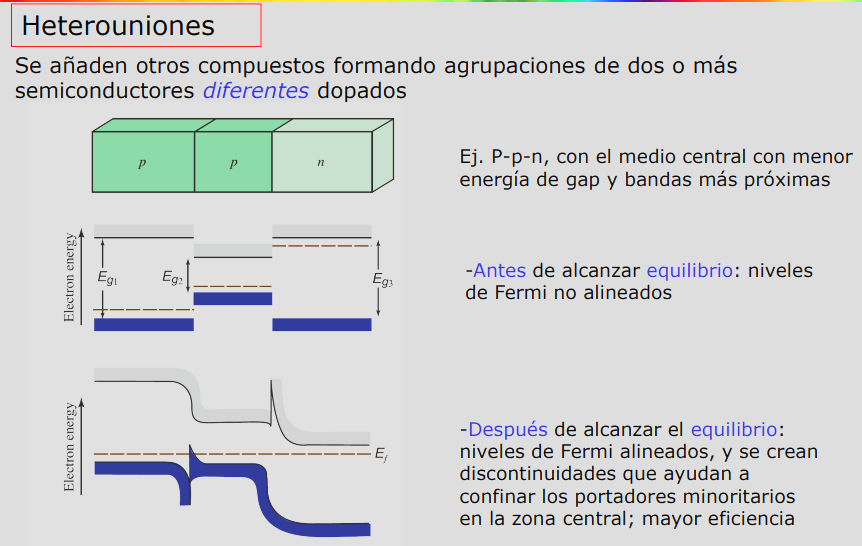
\includegraphics[width=0.7\textwidth]{IMG/pn5.png}
	\end{figure}
	
	\esp
	
	Las uniones descritas hasta ahora en esta subsección estarían formadas por compuestos $p$ y $n$ obtenidos a partir del mismo material semiconductor de partida. Sin embargo, la tecnología dominante en la producción de LEDs utiliza \textbf{heterouniones}, que son agrupaciones de compuestos dopados de diferentes materiales semiconductores. El hecho de utilizar heterouniones hace aumentar la eficiencia del LED, porque se consigue que las cargas estén confinadas en un espacio más pequeño, aumentando la probabilidad de que se produzcan recombinaciones radiativas. El mecanismo de confinamiento de las cargas se produce por la alteración en la distribución de los niveles de Fermi en las distintas zonas de frontera entre los materiales (por ejemplo, en una heterounión tipo $p$-$p$-$n$ se pueden crear barreras con saltos bruscos del nivel de Fermi en las fronteras $p$-$p$ y $p$-$n$ antes de alcanzar el equilibrio, que tras la alineación de los niveles de Fermi al alcanzar el equilibrio, confinen efectivamente los huecos en la banda de valencia y los electrones en la de conducción a la zona intermedia ocupada por el segundo material dopado $p$). Una notación usual para las heterouniones es utilizar combinaciones de letras $p, P$ y $n, N$, donde las mayúsculas denotan el compuesto con mayor energía de gap.
	
	\esp
	
	\begin{figure}[H]
		\centering
		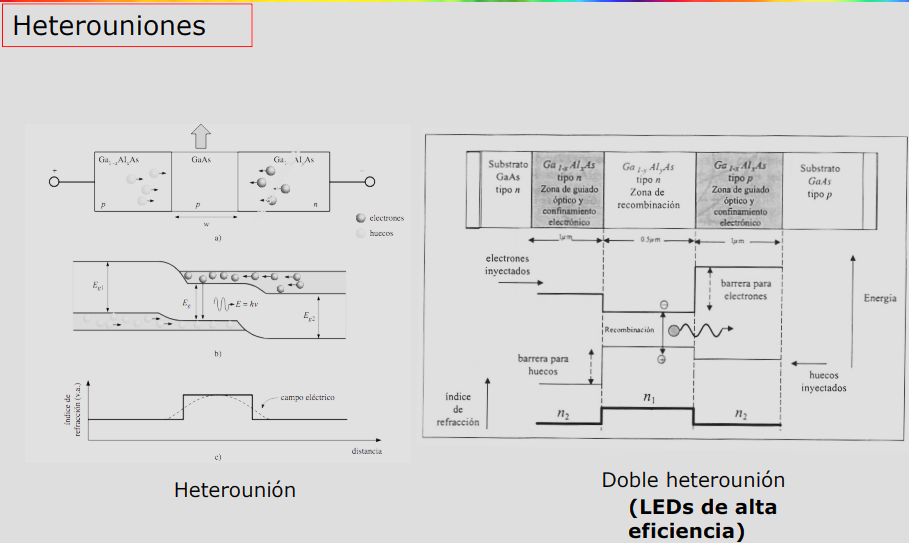
\includegraphics[width=0.7\textwidth]{IMG/pn6.png}
	\end{figure}
	
	\subsection{Claves del mecanismo de emisión. Eficiencia.}
	
	\begin{figure}[H]
		\centering
		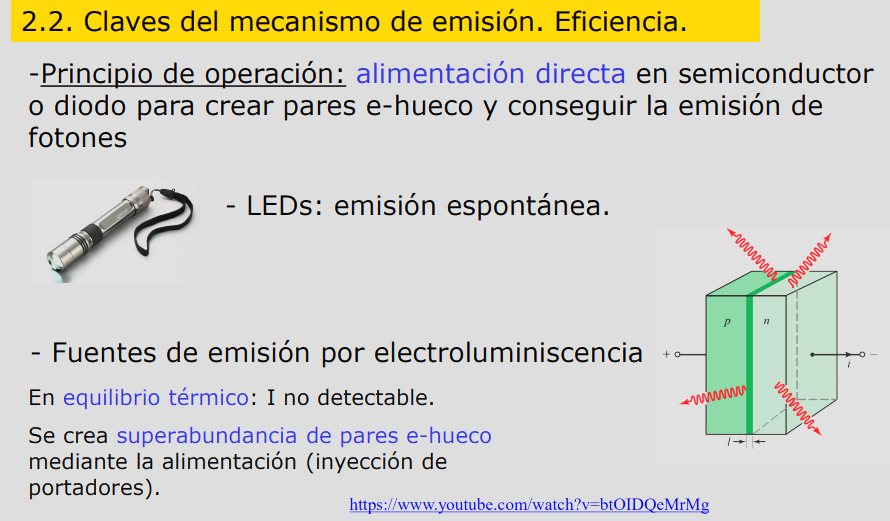
\includegraphics[width=0.7\textwidth]{IMG/pn7.png}
	\end{figure}
	
	\esp
	
	El fenómeno en el cual se basa la emisión LED se llama \textit{electroluminiscencia}. En condiciones de equilibrio térmico, la intensidad de luz emitida en un diodo de semiconductor por recombinación radiativa no es detectable (es del orden de $10^{-20} W/cm^2$). Se necesita, como ya hemos señalado, crear una superabundancia de pares e-hueco en la zona de deplexión para que pueda producirse una emisión apreciable. Esto se realiza mediante el mecanismo denominado \textit{inyección de portadores}.
	
	\esp
	
	\begin{figure}[H]
		\centering
		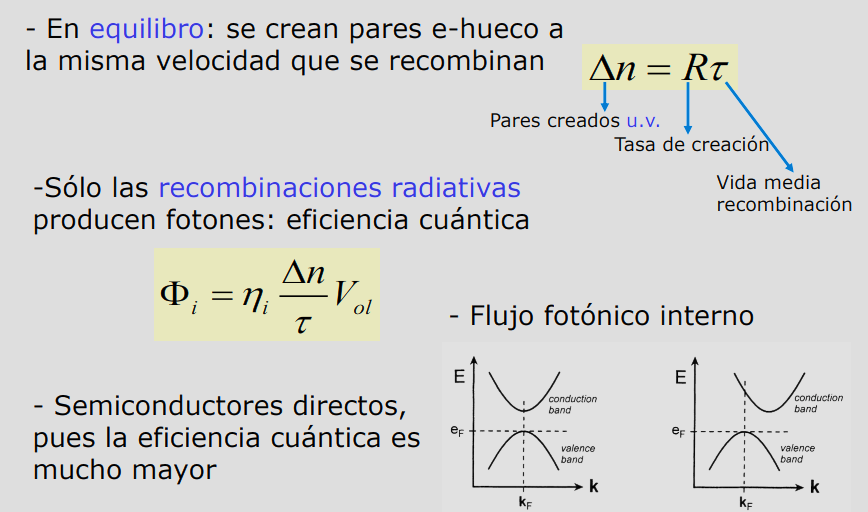
\includegraphics[width=0.7\textwidth]{IMG/pn8.png}
	\end{figure}
	
	\esp
	
	Mediante la alimentación directa, se provoca un movimiento de electrones desde $n$ y de huecos desde $p$ hacia la zona de deplexión. Cuando se alcanza el equilibrio, se crean pares electrón-hueco a la misma velocidad que se recombinan, así que si denominamos $R$ a la tasa de creación de pares por unidad de volumen, y $\tau$ a la vida media de recombinación (por cada recombinación, desaparece un par), el número de pares creados por unidad de volumen $\Delta n$ es el producto $R\tau$. De todos estos pares, sólo los que experimenten recombinaciones radiativas van a producir fotones, y denominando eficiencia cuántica $\eta_i$ a la fracción de recombinaciones radiativas, podemos obtener el flujo de fotones como el producto de la eficiencia cuántica por la tasa de creación por el volumen de la zona de deplexión, con lo que queda proporcional al número de pares creados, lo que resulta lógico.
	
	\esp
	
	\begin{equation}
		\Phi_i = \eta_i \frac{\Delta n}{\tau} V_{ol}
	\end{equation}
	
	\esp
	
	Para los LEDs, se utilizan semiconductores directos, ya que en éstos la eficiencia cuántica es mucho mayor. Por ejemplo, para el $GaAs$ es de 0,5, y para el $Si$ de $10^{-5}$.
	
	\esp
	
	\noindent Vamos a ver ahora algunas de las características más destacadas de los LED.
	
	\esp
	
	\subsubsection{Flujo de fotones generado}
	
	\begin{figure}[H]
		\centering
		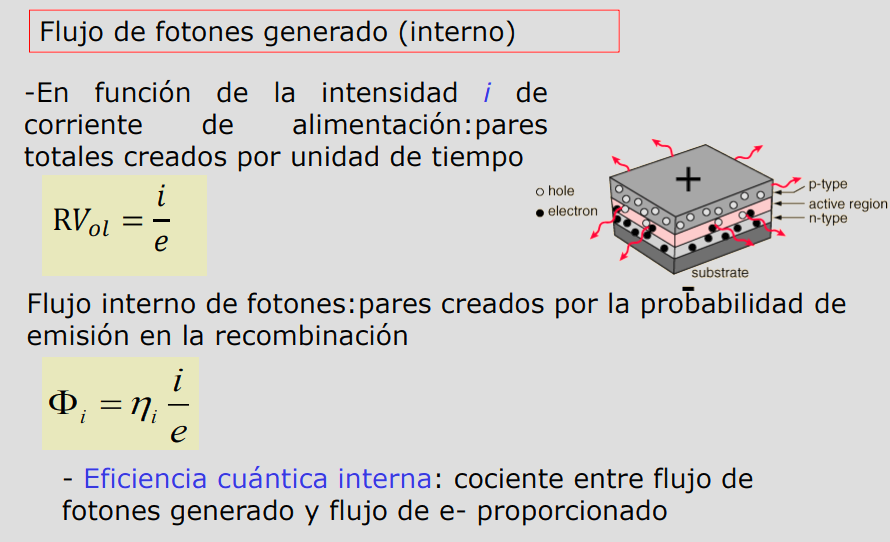
\includegraphics[width=0.7\textwidth]{IMG/pn9.png}
	\end{figure}
	
	\esp
	
	En primer lugar, podemos expresar el flujo interno de fotones (el flujo que hemos calculado en el ejemplo anterior) en función de la intensidad de la alimentación aplicada, ya que la tasa de creación por unidad de volumen $R$ no es más que la intensidad entre la carga del electrón y el volumen. Entonces podemos expresar el número de pares creados por unidad de volumen y el flujo fotónico en función de la intensidad aplicada:
	
	\esp
	
	\begin{align}
		\Delta n &= \frac{i\tau}{e V_{ol}} \\
		\Phi_i &= \eta_i \frac{i}{e}
	\end{align}
	
	\esp
	
	Así, se ve intuitivamente cómo la eficiencia cuántica es el cociente entre el flujo de fotones generado y el flujo de portadores suministrado.
	
	\esp
	
	\subsubsection{Flujo fotónico externo y eficiencia}
	
	\begin{figure}[H]
		\centering
		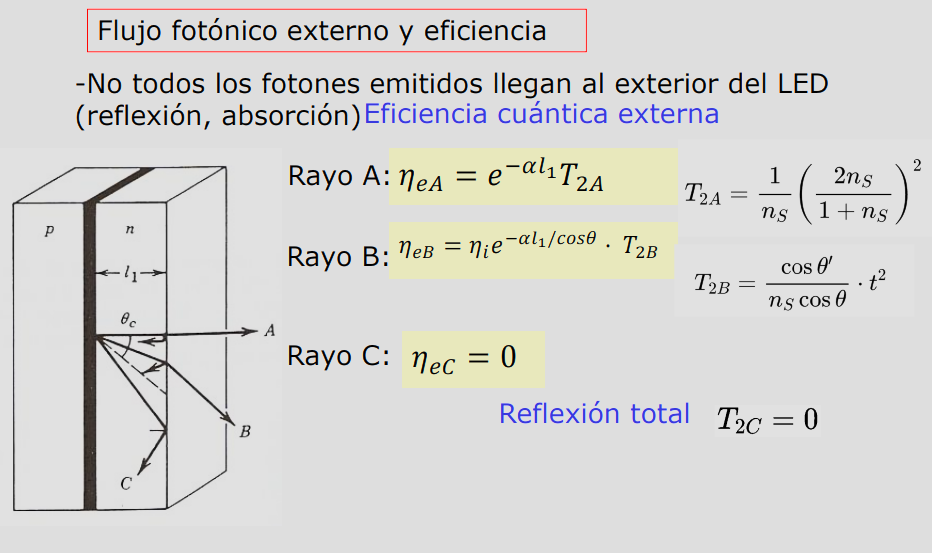
\includegraphics[width=0.7\textwidth]{IMG/pn10.png}
	\end{figure}
	
	\esp
	
	No todos los fotones generados consiguen salir del dispositivo, por lo cual resulta conveniente definir los conceptos de flujo fotónico externo y eficiencia. Por ejemplo, para la dirección de emisión $A$ en la figura 4, tenemos procesos de absorción hasta que se alcanza la superficie del diodo, y el correspondiente factor de transmisión en la interfase con el medio externo (para incidencia normal y si el medio externo es aire, tenemos):
	
	\esp
	
	\begin{equation}
		T_2 = \frac{4n}{(n + 1)^2}
	\end{equation}
	
	\esp
	
	\begin{figure}[H]
		\centering
		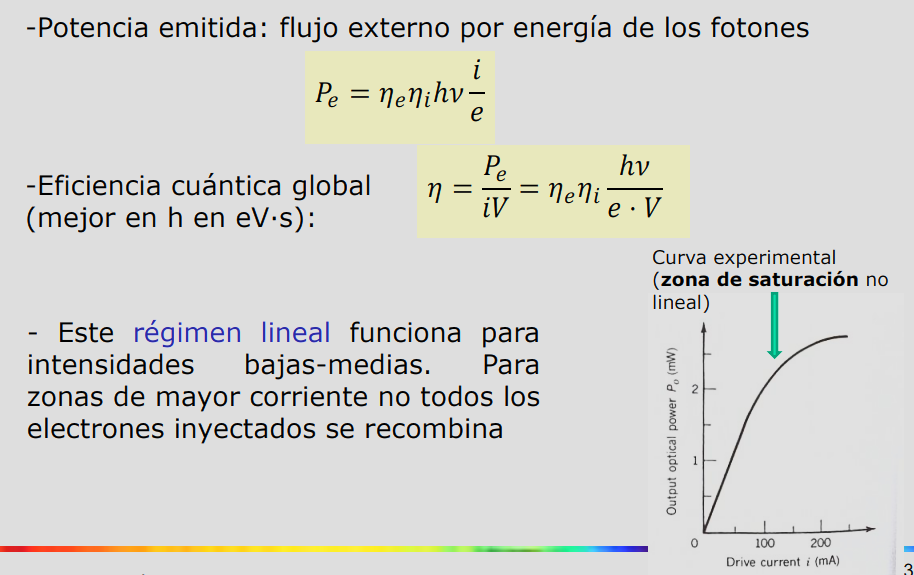
\includegraphics[width=0.7\textwidth]{IMG/pn11.png}
	\end{figure}
	
	\esp
	
	como ya sabemos por Óptica I (relaciones de Fresnel). Estos factores y otros adicionales para otros recorridos (por ejemplo en la dirección $C$ habría reflexión total), se incluyen en el coeficiente de eficiencia cuántica externa $\eta_e = e^{-\alpha l_1} T_2$, que se utilizaría para calcular el flujo fotónico externo igual que hemos visto antes para el flujo interno, y a partir del flujo fotónico externo podemos obtener la expresión para la potencia emitida multiplicando la energía de los fotones por el flujo externo, en función de la intensidad de alimentación:
	
	\esp
	
	\begin{equation}
		P_e = \eta_e h\nu \eta_i \frac{i}{e}
	\end{equation}
	
	\esp
	
	Vemos que según esta expresión, la potencia emitida mantiene una relación lineal con la intensidad suministrada, lo que sólo es cierto en un determinado rango de intensidad de alimentación. Para corrientes mayores, se alcanza la saturación del dispositivo. 
	Usualmente, se define el rendimiento de la fuente como la razón potencia emitida-potencia suministrada, que denominamos en este tema \textit{eficiencia cuántica global del LED}.
	
	\esp
	
	\begin{equation}
		\eta = \frac{P_e}{i V} = \eta_e \eta_i \frac{h\nu}{e \cdot V}
	\end{equation}
	
	\esp
	
	Una de las ventajas de los LED es que tienen un rendimiento luminoso (parámetro relacionado con la percepción visual de la luminosidad de las fuentes de luz) muy elevado, en comparación con muchas de las fuentes convencionales.
	
	\esp
	
	\begin{figure}[H]
		\centering
		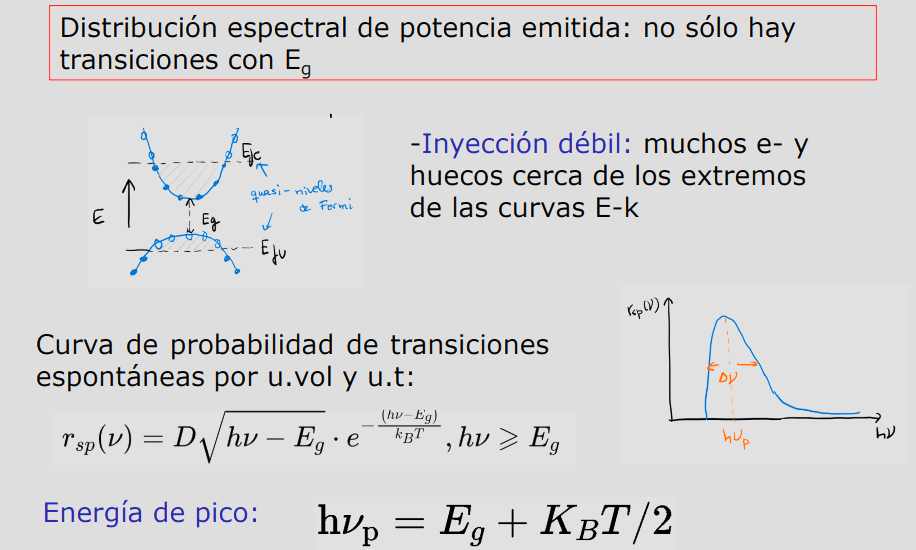
\includegraphics[width=0.7\textwidth]{IMG/pn12.png}
	\end{figure}
	
	\esp
	
	\textbf{Distribución espectral} Nos preguntamos ahora cómo es la curva de emisión espectral típica de un LED, es decir, si representamos la fracción de energía emitida en cada longitud de onda, qué forma tiene esta curva. Dado que se trata de transiciones espontáneas y que la energía de los fotones emitidos está alrededor de un valor definido por el gap del material, no nos resulta extraño que aparezca una curva con forma de pico centrado en la longitud de onda de la transición y con un cierto ancho de banda. La curva de emisión espectral de los LED tiene entonces estas dos características principales: la frecuencia (o longitud de onda, según la variable dependiente de la curva) y la anchura espectral.
	
	\esp
	
	Para obtener la frecuencia de pico, utilizamos la curva de probabilidad de emisiones radiativas en función de la energía de los fotones emitidos ($r_{sp}(h\nu)$), cuya forma teórica puede obtenerse si consideramos una situación simplificada con quasi-niveles de Fermi mucho más distantes de las energías de las bandas que el valor de $k_B T$. Imponemos la condición de máximo, e igualando la primera derivada con respecto a la variable $x = h\nu - k_B T$, obtenemos la expresión para la frecuencia de pico: $h\nu_p = E_g + \frac{k_B T}{2}$. 
	
	\esp
	
	\begin{figure}[H]
		\centering
		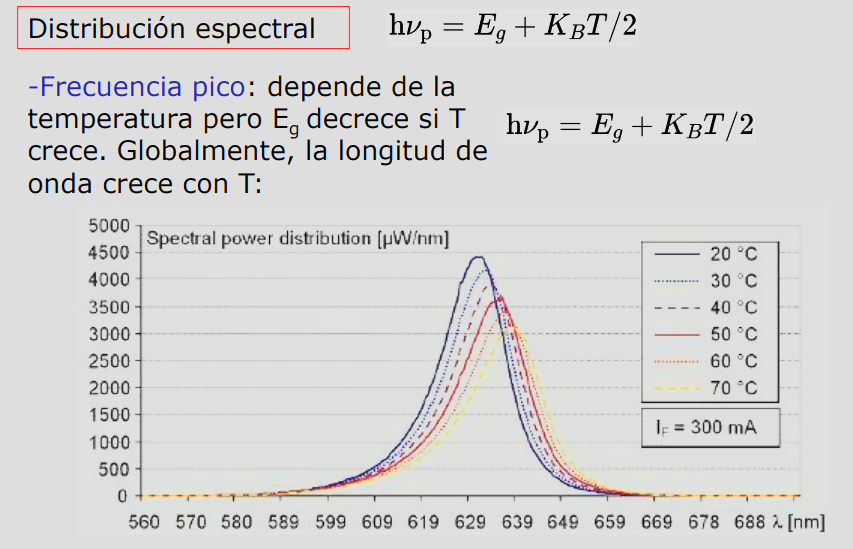
\includegraphics[width=0.7\textwidth]{IMG/pn13.png}
	\end{figure}
	
	\esp
	
	Esta expresión indica que la frecuencia de pico aumentaría con la temperatura, y por tanto la longitud de onda de pico debería disminuir. Sin embargo, el comportamiento observado entre 20 y 70 grados centígrados en los LED es inverso, la longitud de onda de pico crece con la temperatura. Esto es así porque la energía de gap también es dependiente con la temperatura, y decrece conforme crece $T$, compensando el efecto previsto en la ecuación anterior.
	
	\esp
	
	\begin{figure}[H]
		\centering
		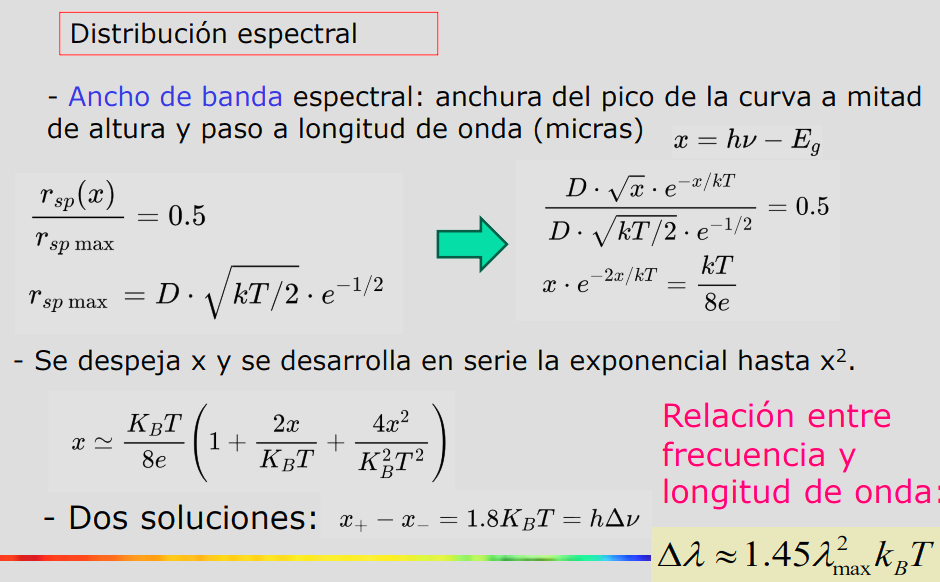
\includegraphics[width=0.7\textwidth]{IMG/pn14.png}
	\end{figure}
	
	\esp
	
	El ancho de banda espectral puede calcularse en función de la longitud de onda de pico utilizando la siguiente expresión:
	
	\esp
	
	\begin{equation}
		\Delta \lambda \approx 1,45 \lambda_{\text{máx}}^2 k_B T
	\end{equation}
	
	\esp
	
	donde $k_B T$ está en $eV$ y el ancho de banda se obtiene en micras. Esta expresión se obtiene a partir de consideraciones sobre distribución energética y probabilidad de transición que requieren algunos conocimientos sobre Física Cuántica y Física de Estado Sólido. 
	
	\esp
	
	\begin{figure}[H]
		\centering
		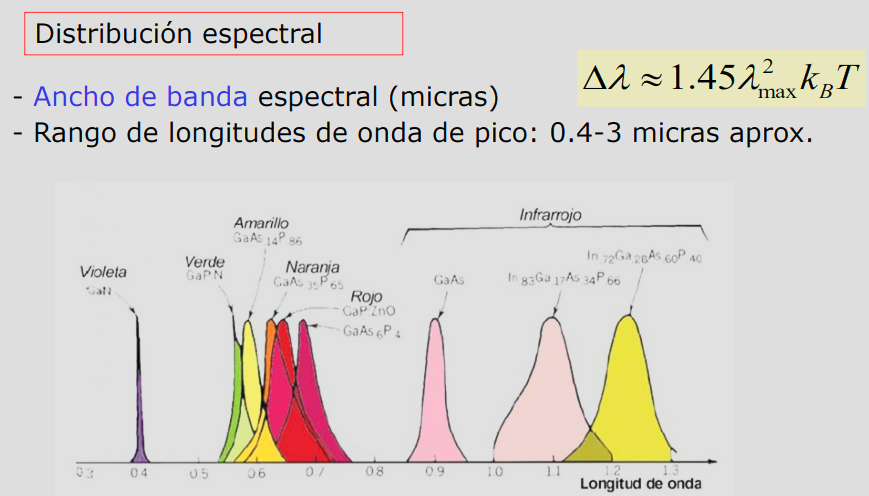
\includegraphics[width=0.7\textwidth]{IMG/pn15.png}
	\end{figure}
	
	\esp
	
	La conclusión, viendo la expresión anterior, es inmediata: para las longitudes de onda mayores (energías de gap menores), el ancho de banda del pico de emisión será también mayor. El rango de longitudes de onda de pico en los LED va entre 0,24 y 4,0 micras aproximadamente. Podemos ver en la figura 5 los diferentes compuestos y la localización de las curvas de emisión en función de la longitud de onda de pico.
	
	\esp
	
	\subsubsection{Materiales de LED}
	
	\begin{figure}[H]
		\centering
		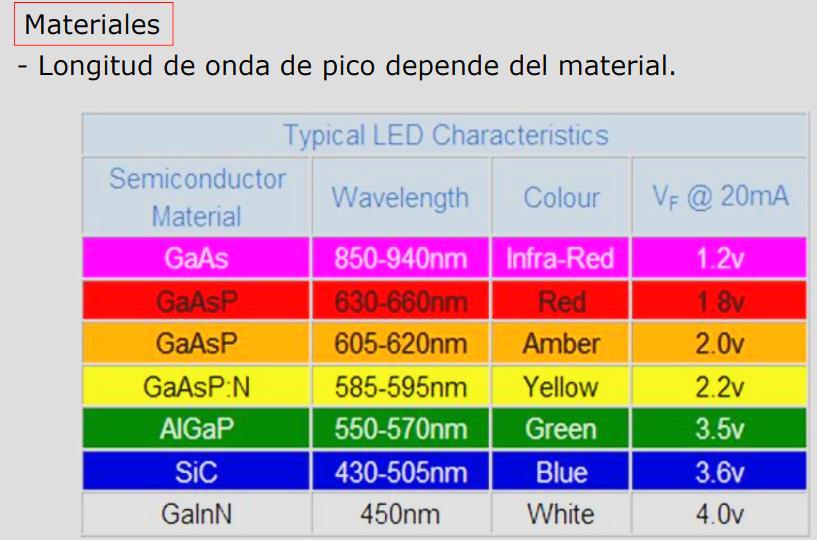
\includegraphics[width=0.7\textwidth]{IMG/pn16.png}
	\end{figure}
	
	\esp
	
	En cuanto a los materiales, ya hemos comentado que la longitud de onda de pico depende del material utilizado. En las longitudes de onda cortas, las condiciones de operación son más restringidas, puesto que la energía de gap es mayor y esto hace decrecer la eficiencia cuántica. 
	
	\esp
	
	\begin{figure}[H]
		\centering
		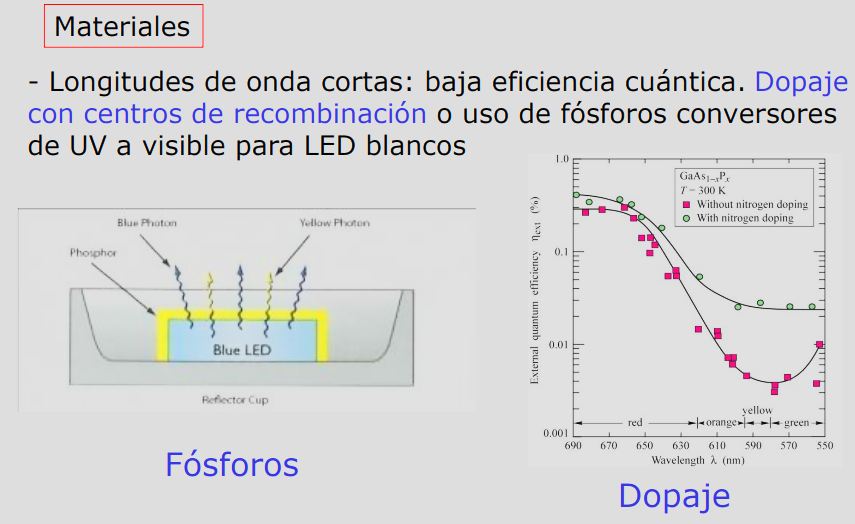
\includegraphics[width=0.7\textwidth]{IMG/pn17.png}
	\end{figure}
	
	\esp
	
	Para atenuar este efecto, suele recurrirse a dopaje con elementos que puedan actuar de centros de recombinación para aumentar la eficiencia (por ejemplo, $GaAs$ dopado con $N$), o bien si tenemos LEDs que emiten en longitudes de onda cortas, podemos utilizar un conversor (fósforo que re-emite en el visible). Esto se hace también en los LED de espectro amplio (LED blancos).
	
	\esp
	
	Vemos en la tabla de las diapositivas de clase algunos tipos de semiconductores habituales en tecnología LED, con las longitudes de onda de pico de emisión y también los voltajes de operación más usuales.
	
	\esp
	
	Como resumen de las características que necesitamos en un material para construir LEDs, podemos decir que los mejores candidatos son compuestos binarios o ternarios, y es fundamental que sean de tipo directo. También deben tener eficiencias cuánticas internas de al menos 0,5.
	
	\subsection{Tipos de LED}
	
	\begin{figure}[H]
		\centering
		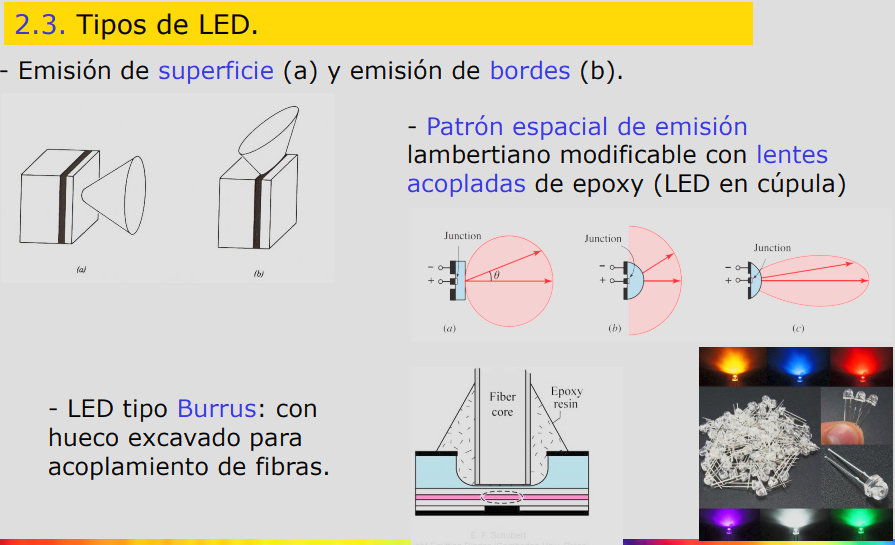
\includegraphics[width=0.7\textwidth]{IMG/tipo.png}
	\end{figure}
	
	\esp
	
	En cuanto a la estructura de los dispositivos, distinguimos en primer lugar entre dos tipos básicos de emisión, \textit{de superficie} (es la que hemos estado viendo en las figuras anteriores), y \textit{de borde} (el LED emite por los bordes de la zona de deplexión). El cono de emisión es entonces más estrecho, como se muestra en la figura 6. En los LED de superficie, se emite desde un lado del diodo, y la luz que va hacia el otro lado es reflejada o reabsorbida para poder crear nuevos pares.
	
	\esp
	En los LED la emisión es de tipo lambertiano (en todas direcciones con intensidad máxima en la normal a la superficie, y mínima en dirección rasante), pero podemos modificar esto con la ayuda de lentes de resina epoxy hemisféricas o parabólicas, si es necesario para obtener patrones de emisión más alargados. Este diseño ya se utiliza menos en general, en especial cuando se requiere algo más de intensidad en la emisión. O bien utilizar fibra óptica para reconducir la emisión y evitar pérdidas, como suele suceder en los LED tipo \textit{Burrus}, como el mostrado en la figura 6 izquierda.
	
	\esp
	
	\begin{figure}[H]
		\centering
		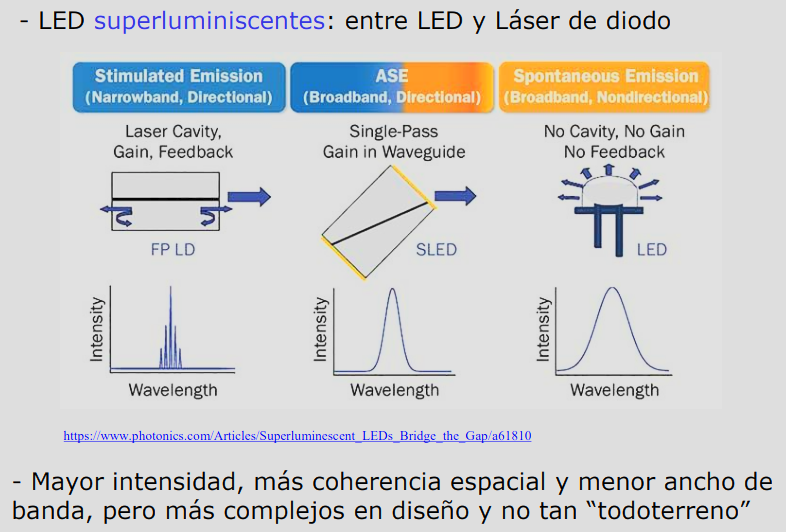
\includegraphics[width=0.7\textwidth]{IMG/tipo2.png}
	\end{figure}
	
	\esp
	
	\begin{figure}[H]
		\centering
		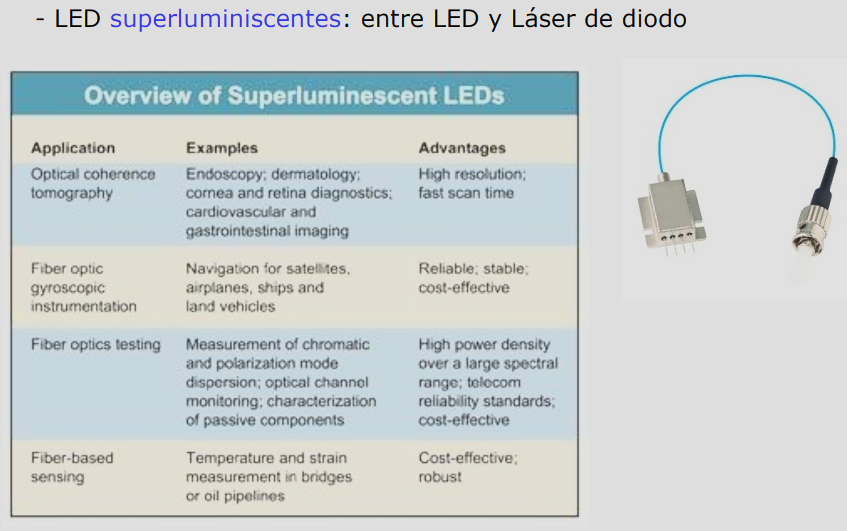
\includegraphics[width=0.7\textwidth]{IMG/tipo3.png}
	\end{figure}
	
	\esp
	
	En los LED \textit{superluminiscentes}, la emisión se produce como consecuencia de un proceso de emisión estimulada mediante un bombeo de fotones (los fundamentos de la emisión estimulada se verán en la sección de láseres), pero sin amplificación de la emisión porque se dejan salir los fotones sin restricciones por un extremo del LED, que es de emisión lateral. Para conseguir esto, se inclina la cavidad resonante. La ventaja es que tienen un ancho de banda espectral más reducido, mayor intensidad y más coherencia espacial, pero la estructura es más compleja generalmente, y con una mayor dependencia con la temperatura.
	
	\esp
	
	\begin{figure}[H]
		\centering
		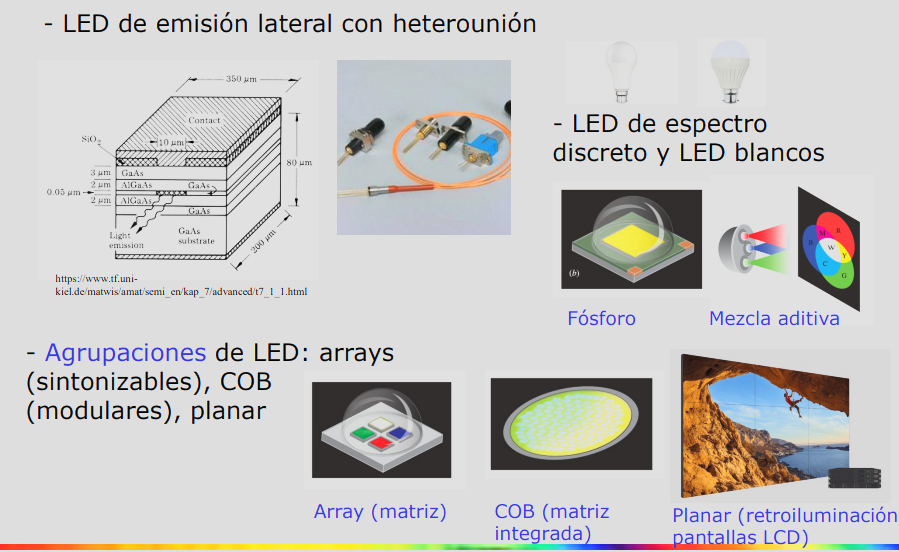
\includegraphics[width=0.7\textwidth]{IMG/tipo4.png}
	\end{figure}
	
	\esp
	
	En cuanto a la distribución de longitudes de onda de emisión, podemos distinguir entre LEDs \textit{de espectro discreto} y LEDs \textit{blancos}. La tecnología para generar luz blanca con LEDs puede basarse en la adición de un estrato de material fosforescente (que ya mencionamos en la subsección anterior), o bien en el uso de varios LEDs (suelen ser rojo, verde y azul) para generar luz blanca por un proceso de mezcla aditiva, en el que el espectro generado es la envolvente de los espectros de los LED individuales, que necesitan tener ancho de banda relativamente elevado.
	
	\esp
	Desde el punto de vista de la distribución espacial, como veremos en la sección de aplicaciones también, es muy común construir \textit{agrupaciones de LED} para conseguir una mayor intensidad y una distribución espacial más homogénea. Las agrupaciones más comunes son en forma de matriz (\textit{array}), o bien \textit{Chip On Board} (COB), en la que los LED se montan con un circuito común e incluyendo fósforos y difusores también. Los llamados \textit{LED planos} se utilizan también en formato matriz, para servir de fuentes traseras de retroiluminación en pantallas de gran formato, aunque la tecnología evoluciona hacia las pantallas menos voluminosas igualmente, por el ahorro energético que supone retroiluminar con LED.
	
	\esp
	Los LED son dispositivos de muy bajo consumo y rendimientos superiores a otras fuentes convencionales (las corrientes suministradas son del orden de $mA$), así que agruparlos para formar configuraciones extensas puede suponer una ventaja. Además, tienen una respuesta muy rápida a la modulación (incluso de $GB/s$), lo que se presta bien a utilizarlos en iluminación cambiante en el tiempo, como las figuras en movimiento que vemos en los semáforos de peatones o los letreros luminosos.
	
	\subsubsection{Aplicaciones de los LED}
	
	Vamos a describir las diferentes aplicaciones dividiéndolas en función del criterio de longitud de onda de emisión, y considerando tres rangos: visible, infrarrojo y ultravioleta.
	
	\esp
	\subsubsection{Aplicaciones de LED en visible}
	
	\begin{figure}[H]
		\centering
		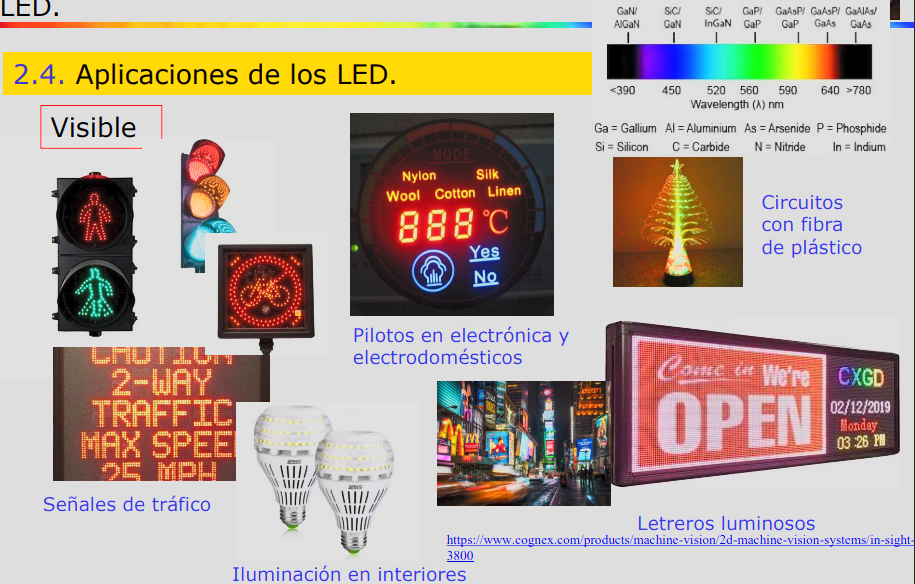
\includegraphics[width=0.7\textwidth]{IMG/aplic.png}
	\end{figure}
	
	\esp
	
	Los LED de $GaAsP$, dopados adicionalmente con Nitrógeno para conseguir un aumento en la energía del gap y mover la emisión inicial infrarroja al visible, se utilizan bastante en indicadores y pilotos en electrónica de consumo, por su bajo coste de fabricación.
	
	\esp
	Los LED de $AlInGaP$ emiten de forma bastante eficiente en el visible, y son los utilizados mayoritariamente en señales de tráfico (semáforos, señales de peligro) y letreros luminosos, especialmente en la zona de medias-altas longitudes de onda. En heteroestructura con $InGaP$ se utiliza a veces en circuitos de fibra de plástico que trabajan con longitud de onda roja de 650 nm y suelen incorporar también reflectores con estructura tipo multicapa de $AlAs$ y $AlGaAs$, para aumentar la potencia emitida. Para fuentes de alta intensidad entre 400 y 580 nm, se opta por LEDs de $InGaN$, bien en heteroestructura, o en disposición tipo \textit{pozo cuántico}, que se describirá brevemente en la siguiente sección.
	
	\esp
	\subsubsection{Aplicaciones de LED en infrarrojo}
	
	\begin{figure}[H]
		\centering
		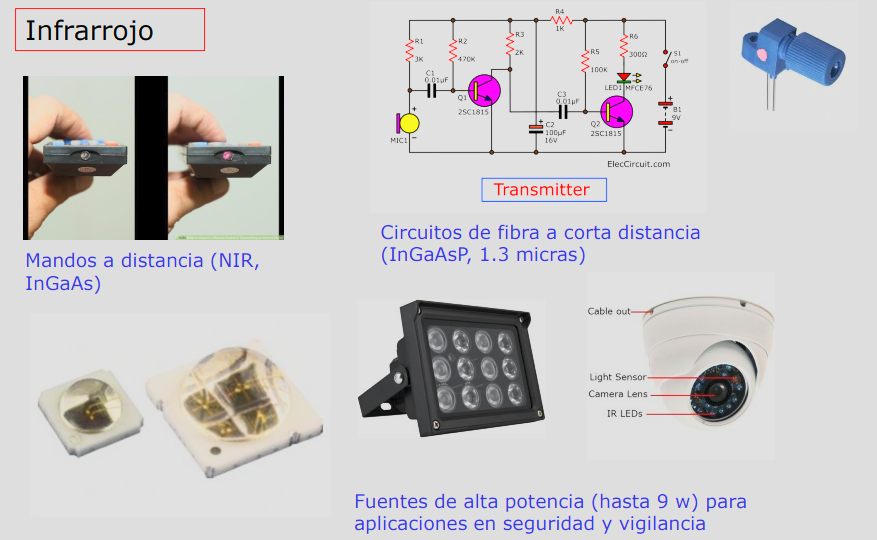
\includegraphics[width=0.7\textwidth]{IMG/aplic2.png}
	\end{figure}
	
	\esp
	
	Los LED de $GaAsP$ o bien $InGaAs$ pueden utilizar su emisión original en infrarrojo para emitir las señales en mandos de control remoto (por eso, somos capaces de ver estas señales con las cámaras de algunos móviles, que no filtran la región del infrarrojo cercano).
	
	\esp
	El compuesto cuaternario $InGaAsP$ puede generar radiación cercana a 1,3 $\mu m$, y a veces se utilizan LEDs de este tipo para comunicaciones por fibra que no sean de largo recorrido ni muy rápidas, ya que en ese caso es mejor usar láseres de diodo o de fibra. La configuración habitual es tipo Burrus con conexión de fibra, como se muestra en la figura 6 izquierda, o bien se incorpora una lente para colimar el haz y acoplarlo posteriormente a la fibra.
	
	\esp
	Las fuentes LED más potentes en infrarrojo se consiguen con compuestos cuaternarios en hetero-unión o bien haciendo uso de estructuras de tipo \textit{pozo cuántico}.
	
	\esp
	\subsubsection{Aplicaciones de LED en Ultravioleta}
	
	\begin{figure}[H]
		\centering
		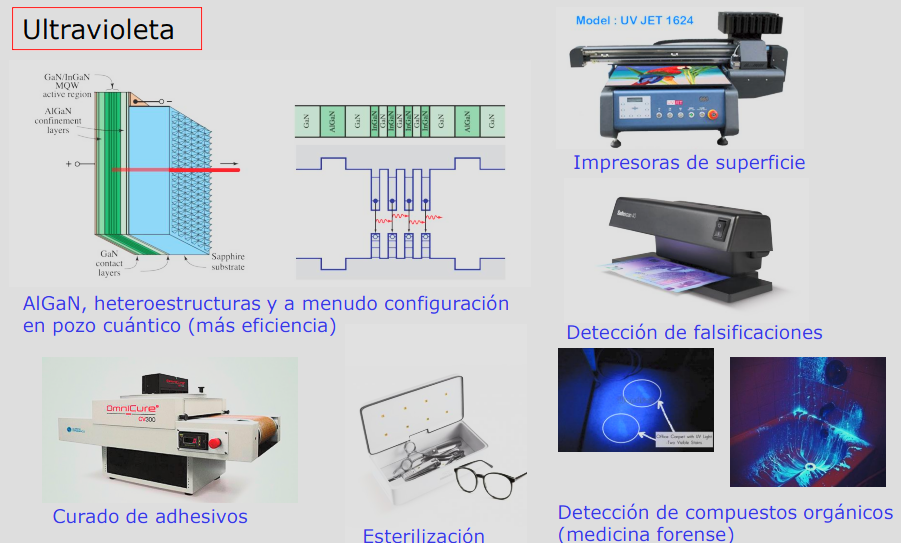
\includegraphics[width=0.7\textwidth]{IMG/aplic3.png}
	\end{figure}
	
	\esp
	
	Los LED que emiten ultravioleta suelen ser de $AlGaN$ (que cubre entre 200 y 366 nm). Con energías más elevadas de gap, es más difícil controlar la eficiencia, así que suelen utilizarse configuraciones de hetero-unión tipo pozo cuántico, y se montan sobre zafiro transparente con tallado en forma de pirámides, para incrementar el número de fotones que pueden ser extraídos del material del LED. Las aplicaciones son muchísimas: a partir de 315 nm se utilizan en impresoras, detección de falsificaciones (en billetes, entradas y documentos de identidad, por ejemplo) y para curar algunos materiales como tintas, recubrimientos y adhesivos. Entre 100 y 280 nm, se utilizan para esterilizar, en sistemas de tratamiento de aguas, y también en medicina forense para detectar compuestos orgánicos debido a su fluorescencia. También en comunicaciones encubiertas a corta distancia o \textit{non line-of-sight} (NLOS).
	
	\section{Láser}
	
	\begin{figure}[H]
		\centering
		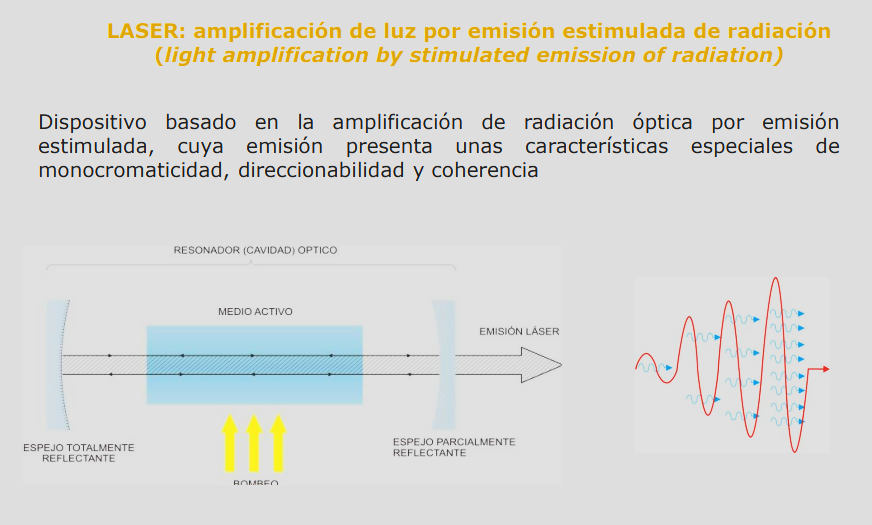
\includegraphics[width=0.7\textwidth]{IMG/laser.png}
	\end{figure}
	
	\esp
	
	Para comprender el proceso de emisión en un láser, es necesario introducir conceptos básicos sobre la interacción de la radiación con la materia relativos a los procesos de absorción y emisión de fotones.
	
	\esp
	
	\subsection{Emisión estimulada}
	
	\begin{figure}[H]
		\centering
		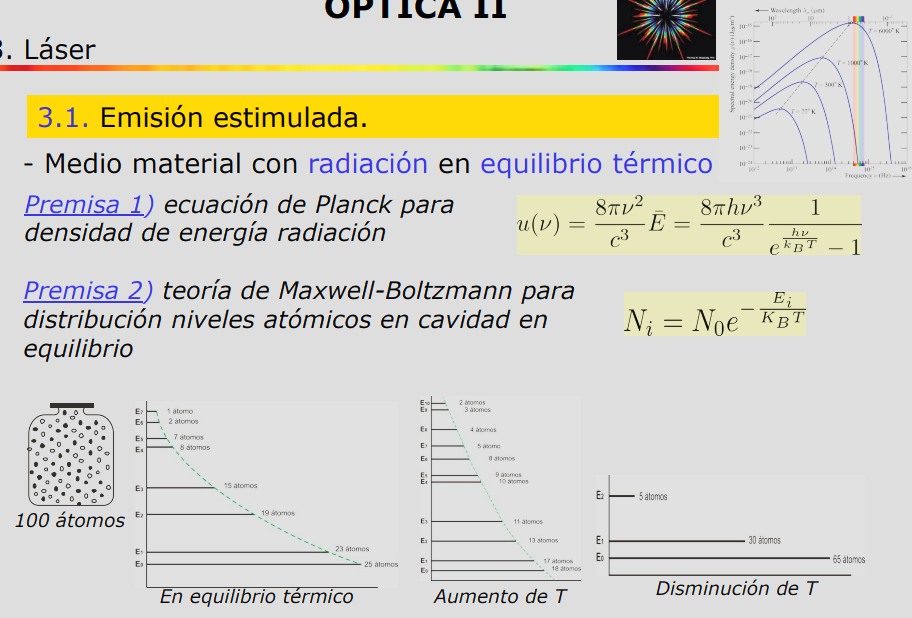
\includegraphics[width=0.7\textwidth]{IMG/laser2.png}
	\end{figure}
	
	\esp
	
	Einstein desarrolló en 1916-1917 un modelo teórico muy sencillo y elegante para describir los procesos que tienen lugar en un medio material en equilibrio con radiación e.m. Vamos a ver el proceso de construcción del modelo a partir de las hipótesis que se fueron formulando, y que llevaron a la suposición de Einstein de que debía existir un proceso en el medio no conocido hasta entonces y que se llamó \textit{emisión estimulada}.
	
	\esp
	Partimos de algunos resultados conocidos, fundamentalmente la ecuación de Planck para la densidad de energía del cuerpo negro (radiación en una cavidad en equilibrio a temperatura $T$) expresada en función de la frecuencia:
	
	\esp
	\begin{equation*}
		u(\nu) = \frac{8\pi\nu^2}{c^3}\bar{E} = \frac{8\pi h\nu^3}{c^3}\frac{1}{e^{\frac{h\nu}{k_B T}} - 1}
	\end{equation*}
	
	\esp
	$K_B$ es la constante de Boltzmann.
	También adopta Einstein como premisa la distribución de Maxwell-Boltzmann para el número de átomos por unidad de volumen en estado excitado en una cavidad llena de gas a temperatura $T$, según la expresión siguiente en función de la energía $E_i$ del estado excitado:
	
	\esp
	\begin{equation*}
		N_i = N_0 e^{-\frac{E_i}{k_B T}}
	\end{equation*}
	
	\esp
	
	\begin{figure}[H]
		\centering
		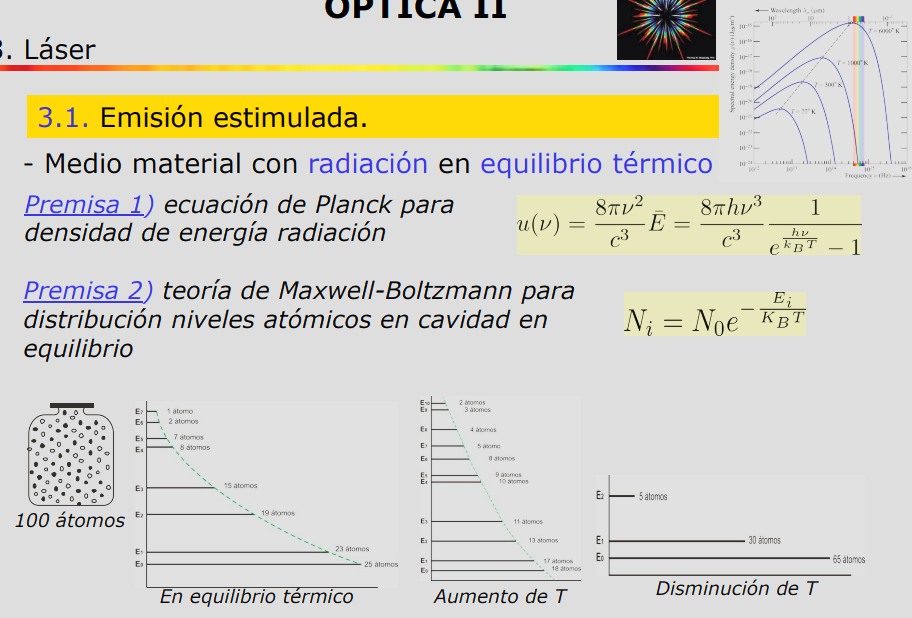
\includegraphics[width=0.7\textwidth]{IMG/laser2.png}
	\end{figure}
	
	\esp
	
	Lo que viene a decirnos esta ecuación es algo muy intuitivo: cuanto mayor sea la energía de un estado excitado, menos átomos tendremos con electrones ocupando el mismo, o de otra forma, que se tiende de forma natural a ocupar los estados de menor energía. Esto lo vemos esquematizado en la figura 7.
	
	\esp
	
	\begin{figure}[H]
		\centering
		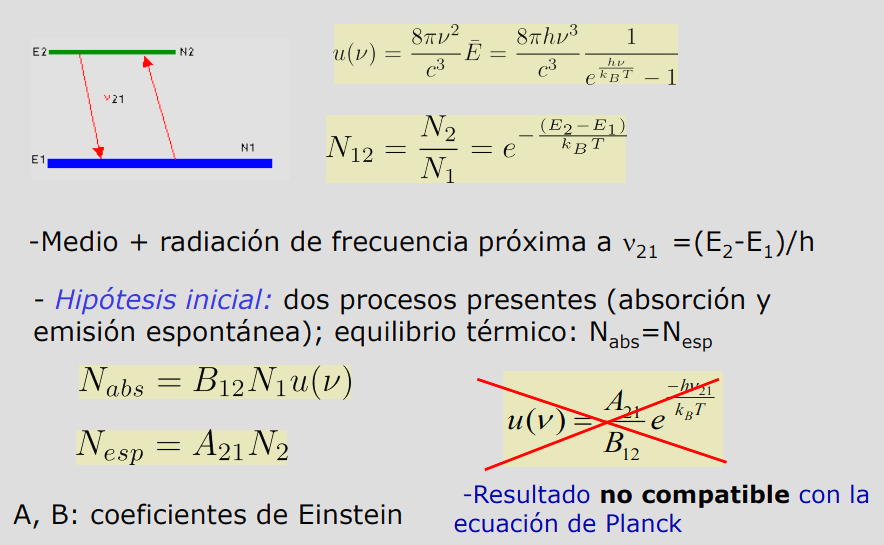
\includegraphics[width=0.7\textwidth]{IMG/laser3.png}
	\end{figure}
	
	\esp
	Si consideramos dos estados con energías $E_1$ y $E_2$, con $E_2 > E_1$, es muy fácil obtener una relación entre el número de átomos con electrones ocupando los niveles $E_2$ y $E_1$ utilizando la distribución de Maxwell-Boltzmann, y este cociente queda en función de la frecuencia propia de la transición entre los estados 2 y 1, teniendo en cuenta que la energía de un posible fotón desprendido por esta transición sería $h\nu_{21} = E_2 - E_1$.
	
	\esp
	\begin{equation*}
		N_{12} = \frac{N_2}{N_1} = e^{-\frac{(E_2 - E_1)}{K_B T}}
	\end{equation*}
	
	\esp
	Si este medio en equilibrio en la cavidad a temperatura $T$ se ve sometido a una radiación de densidad $u(\nu)$ con frecuencias alrededor de la frecuencia de transición $\nu_{21}$, podrán producirse cambios de estado del nivel 1 al 2 por \textit{absorción} de fotones, cuyo número resultará proporcional al producto $N_1 u(\nu)$.
	Llamaremos $B_{12}$ al coeficiente de proporcionalidad. Entonces, el número de fotones absorbidos será:
	
	\esp
	\begin{equation*}
		N_{abs} = B_{12} N_1 u(\nu)
	\end{equation*}
	
	\esp
	También pueden producirse \textit{transiciones espontáneas} hacia abajo, es decir, del nivel 2 al 1, con la emisión del fotón correspondiente. El número de estas transiciones será proporcional a $N_2$, pero independiente de la densidad de energía de la radiación presente, puesto que se trata de transiciones \textit{usuales} espontáneas. Denominamos $A_{21}$ a la constante de proporcionalidad. Entonces:
	
	\esp
	\begin{equation*}
		N_{esp} = A_{21} N_2
	\end{equation*}
	
	\esp
	Si el sistema está en equilibrio y tenemos sólo estos dos procesos presentes, el número excitaciones (transiciones hacia el nivel 2 desde el 1) debe igualar al de decaimientos (transiciones del nivel 2 al nivel 1), puesto que si no se vería afectado el balance energético del sistema. Igualando entonces $N_{abs}$ y $N_{esp}$, despejando la densidad de energía, y utilizando la relación entre el número de átomos $N_2$ y $N_1$ que hemos deducido antes, se llega entonces fácilmente a una expresión para la densidad de energía e.m.:
	
	\esp
	\begin{equation*}
		u_2(\nu) = \frac{A_{21}}{B_{12}} e^{-\frac{h\nu_{21}}{K_B T}}
	\end{equation*}
	
	\esp
	que como vemos no coincide con la distribución propuesta por Planck que hemos adoptado como premisa.
	Así que esta expresión no resulta válida, y debemos habernos dejado algún proceso adicional sin considerar. 
	
	\esp
	
	\begin{figure}[H]
		\centering
		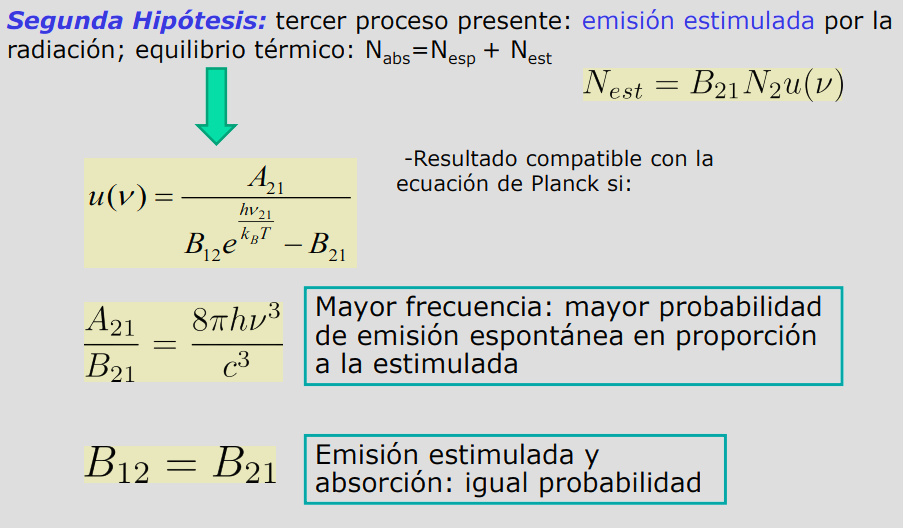
\includegraphics[width=0.7\textwidth]{IMG/laser4.png}
	\end{figure}
	
	\esp
	
	Einstein propuso que este proceso sería de \textit{emisión estimulada}, es decir, que habría transiciones del nivel 2 al 1 condicionadas por la presencia de radiación e.m. de frecuencia coincidente con la de la transición ($\nu_{12}$). El número de emisiones estimuladas será proporcional a $N_2$ y a la densidad de energía de radiación, $u(\nu)$. Denominemos $B_{21}$ al coeficiente de proporcionalidad. Entonces:
	
	\esp
	\begin{equation*}
		N_{est} = B_{21} N_2 u(\nu)
	\end{equation*}
	
	\esp
	Volvemos ahora a plantear la igualdad que expresa la situación de equilibrio energético: $N_{esp} + N_{est} = N_{abs}$ y despejamos de nuevo la densidad de energía, con lo que nos queda una expresión que sí puede resultar compatible con la ecuación de Planck para la densidad de energía, siempre que se cumplan dos condiciones:
	
	\esp
	\begin{itemize}
		\item que el cociente $\frac{A_{21}}{B_{21}}$ sea inversamente proporcional al cubo de la longitud de onda en el vacío.
		\item que las probabilidades de emisión estimulada $B_{21}$ y absorción $B_{12}$ sean iguales.
	\end{itemize}
	
	\esp
	De la primera condición se deduce que la probabilidad de emisión estimulada frente a la transición espontánea es menor conforme crece la frecuencia. Así que si pensamos en aprovechar la radiación por emisión estimulada, sería más difícil desarrollar un instrumento para ello en el rango de frecuencias altas (rayos X, UV). Esto efectivamente es cierto, aunque se han logrado resolver las dificultades que entraña. También por ello resultó más fácil desarrollar el máser que el láser.
	
	\esp
	
	\begin{figure}[H]
		\centering
		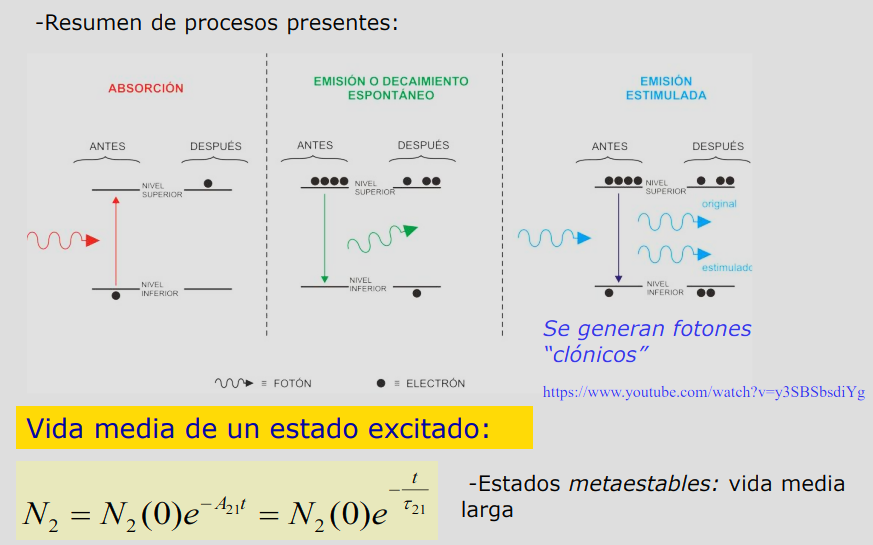
\includegraphics[width=0.7\textwidth]{IMG/laser5.png}
	\end{figure}
	
	\esp
	
	La segunda condición ya la hemos comentado: las probabilidades de absorción y de emisión estimulada son iguales. El proceso que predomine en el sistema dependerá de las proporciones relativas de $N_1$ y $N_2$. Si consideramos la variación con el tiempo del número de átomos en el estado excitado que decaigan por emisión espontánea, es muy fácil llegar a una ecuación diferencial cuya solución nos dice que $N_2$ decrece exponencialmente con el tiempo:
	
	\esp
	\begin{equation*}
		N_2 = N_2(0) e^{-A_{21}t} = N_2(0) e^{-\frac{t}{\tau_{21}}}
	\end{equation*}
	
	\esp
	La tasa de decaimiento es proporcional a $A_{21}$, y por tanto en un tiempo $\frac{1}{A_{21}}$ la población desciende en un factor $e$. A dicho tiempo denominamos \textit{vida media} del estado. Existen determinados estados con mucha mayor vida media que otros situados a su alrededor, y que se denominan \textit{metaestables}. La existencia de este tipo de estados veremos que es clave para que un medio pueda producir emisión láser.
	
	\esp
	Un aspecto muy importante de la emisión estimulada es que el fotón emitido tiene exactamente las mismas características que el inductor en cuanto a fase, frecuencia, polarización, etc. Es como si en el proceso de emisión estimulada, se generasen \textit{clones} de los fotones que estimulan la emisión. Esto se muestra gráficamente en la figura 8, frente a las transiciones espontáneas que emiten fotones de características mucho menos uniformes.
	
	\esp
	Podemos entonces pensar que lo interesante sería descartar los fotones de emisión espontánea y quedarse con los \textit{clones} de emisión estimulada, amplificando así progresivamente la radiación en la cavidad y obteniendo una emisión altamente coherente. Esta es la idea clave que subyace en el diseño del láser. Pero para ello, debemos asegurar en primer lugar que haya el suficiente número de electrones excitados, porque en la situación usual de equilibrio térmico, ya sabemos que la gran mayoría van a estar ocupando los niveles de menor energía, lo que no es favorable para el proceso de emisión estimulada. En la siguiente sección, vamos a ver qué resulta necesario para hacer funcionar el mecanismo de emisión del láser.
	
	\printbibliography[title={Bibliografía}]
\end{document}